\documentclass[a0paper,portrait]{baposter}

\usepackage[utf8]{inputenc}
\usepackage[T1]{fontenc}
\usepackage[table]{xcolor}
\usepackage{amsmath}
\usepackage{array}
\usepackage{colortbl}
\usepackage{geometry}
\usepackage{graphicx}
\usepackage{lmodern}
\usepackage{lipsum, graphicx}
\usepackage{newpxtext, newpxmath}
\usepackage{tcolorbox}
\usepackage{wasysym}
\usepackage{wrapfig}
\usepackage{xcolor}


\selectcolormodel{cmyk}

\graphicspath{{figures/}} % Directory in which figures are stored

\newcommand{\compresslist}{%
\setlength{\itemsep}{0pt}%
\setlength{\parskip}{1pt}%
\setlength{\parsep}{0pt}%
}

\newenvironment{boenumerate}
    {\begin{enumerate}\renewcommand\labelenumi{\textbf\theenumi.}}
    {\end{enumerate}}
\begin{document}

\definecolor{major_color_1}{HTML}{E64626}       % #E64626
\definecolor{major_color_2}{HTML}{E64626}       % #E64626
\definecolor{table_color_1}{HTML}{BBE6DC}       % #BBE6DC
\definecolor{table_color_2}{HTML}{F0FAF5}       % #F0FAF5
\definecolor{table_color_3}{HTML}{E6F5EB}       % #E6F5EB
\definecolor{dark_blue}{HTML}{285FB4}           % #285FB4
\definecolor{color_me}{HTML}{E6F0FA}            % #F0F5FF

\begin{poster}
{
    grid=false,
    headerborder=open,      % Adds a border around the header of content boxes
    colspacing=4pt,         % Column spacing
    bgColorOne=white,
    bgColorTwo=white,
    borderColor=major_color_1,    % Border color
    headerColorOne=major_color_2,
    headerColorTwo=major_color_2,
    headerFontColor=white,
    boxColorOne=white,
    textborder=rounded,
    eyecatcher=false,
    headerheight=0.07\textheight,
    headershape=rounded,
    headershade=plain,
    headerfont=\large\textbf,
    linewidth=1pt,
    columns=5
}{}
%%%%% Title and author
% {
%     {\vspace{15pt}\Large{Electronic and Optical Properties of Heterostructures of Graphene \par and 2D Semiconducting Boron carbides}}
% }
% {
%     \vspace{-20pt}
%     \par Lu Niu, Oliver Conquest, Carla Verdi, Catherine Stampfl
%     \par\footnotesize{School of Physics, The University of Sydney, Sydney, 2006 Australia}
% }
{
    \vspace{20pt}
    \begin{center}\begin{minipage}{500pt}
        \Large{Electronic and Optical Properties of Heterostructures of Graphene and 2D Semiconducting Boron carbides}
        \begin{center}
            \par\vspace{-5pt}\large{Lu Niu, Oliver Conquest, Carla Verdi, Catherine Stampfl}
            \par{School of Physics, The University of Sydney, Sydney, 2006 Australia}
        \end{center}
    \end{minipage}
    \begin{minipage}{60pt}
        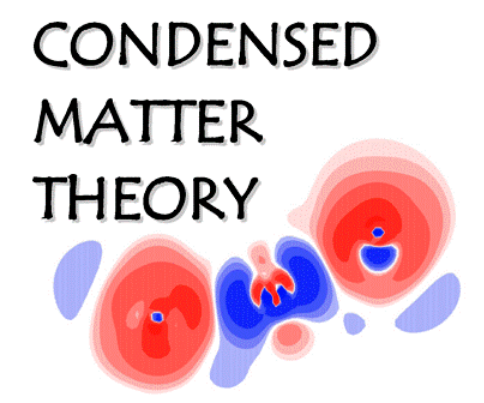
\includegraphics[width=\linewidth]{poster_figures/USyd_CMT.png}
    \end{minipage}
    \begin{minipage}{60pt}
        
\includegraphics[width=\linewidth]{poster_figures/USyd_logo.png}
    \end{minipage}\end{center}
}

%%%% Introduction
% \headerbox{Introduction}{name=introduction, column=0, row=0, span=3}{
% }

\headerbox{Abstract}{name=box_1, column=0, span=2}{
\footnotesize{
\par Integration of dissimilar two-dimensional (2D) materials is essential for nanoelectronics applications. 
For conventional 2D materials derived from bulk-layered crystals, vertical heterostructures can be realized by mechanical stacking [1].
Graphene has excellent electrical conductivity, mechanical and thermal properties, and high light transmittance in the visible light–infrared area.
It has found applications in e.g. solar cells, lighting, and touch screens.
However, graphene has been limited due to its zero band gap.
One of the methods used to expand the application of graphene is to form heterostructures.
Stacking different 2D materials together can form a double-layer or even multi-layer artificial materials that are maintained by van der Waals interactions [2]. Such materials are known as van der Waals heterojunctions.
A wide range of physical properties can be obtained by such stacking, making van der Waals heterojunctions even more important than the 2D material itself.
\par A current research theme is investigating the prospect of developing plasmonic devices using 2D semiconductors [3]. Plasmonic modes in each class of van der Waals semiconductors have their own peculiarities, along with potential technological capabilities. Graphene (G) has an extremely high quantum efficiency for light–matter interactions, is strongly optically nonlinear and contains plasmons with unusual properties that are tunable and adjustable.
Carbon and boron can mix to form numerous 2D compounds with strong covalent bonds, yet very few possess a bandgap for functional applications.
Graphene-like BC\textsubscript{3} has been confirmed experimentally and is found to be semiconducting with an indirect bandgap of around 0.5 eV.
Calculations have shown that nanostructures of graphene-like BC\textsubscript{3} possess preferable absorbance in the visible region and by changing the size of the nanostructure, the resonance peak position of the absorption spectrum can be effectively regulated [4].
\par In the present work we combine these two materials to study the electronic and optical properties of a series of graphene/boron-carbide heterostructures, starting with G/BC\textsubscript{3}.
We use density functional theory as implemented in the VASP (Vienna Ab initio Simulation Package) software and report the electronic band structure, density of states, complex dielectric function and the absorption spectra, and compare them with those of the respective isolated monolayers. Our results show potential metallic properties of G-BC\textsubscript{3} which needs to be confirmed by further calculations.
The adsorption spectra also demonstrate characteristic peaks around 1200nm, 700nm, and between 350nm to 250nm.
\vspace{5pt}
\par[1] K. S. Novoselov, A. Mishchenko, A. Carvalho, A. H. Castro Neto, 2D materials and van der Waals heterostructures, Science 353, 9439 (2016).
\par[2] Bin Qiu, Xiuwen Zhao, Guichao Hu, Weiwei Yue, Junfeng Ren and Xiaobo Yuan, Optical Properties of Graphene/MoS2 Heterostructure: First Principles Calculations, Nanomaterials, 8, 962 (2018).
\par[3] A. Agarwal, M. S. Vitiello, L. Viti, A. Cupolillo and A. Politano, Plasmonics with two-dimensional semiconductors: from basic research to technological applications, Nanoscale,10, 8938 (2018).
\par[4] J. Chen, X.-L. Cheng, H. Zhang, Plasmon Excitation in BC\textsubscript{3} Nanostructures from First Principles, Plasmonics, 14, 109 (2019).

}
}

\headerbox{}{name=pics, boxheaderheight=10pt, column=0, span=2, below=box_1}{
\begin{minipage}{0.56\linewidth}
    \footnotesize{
        \par (a) Scanning Tunneling Microscopy images of a BC\textsubscript{3} sheet with a honeycomb structure. 
        \par (b) clearly shows that the moire-like patterns uniformly covered the entire surface. 
        These have been grown via carbon substitution on NbB\textsubscript{2}.
        \vspace{5pt}\par [5] Solid State Communications 136 (2005) 22–25}
    \end{minipage}
    \begin{minipage}{0.42\linewidth}
        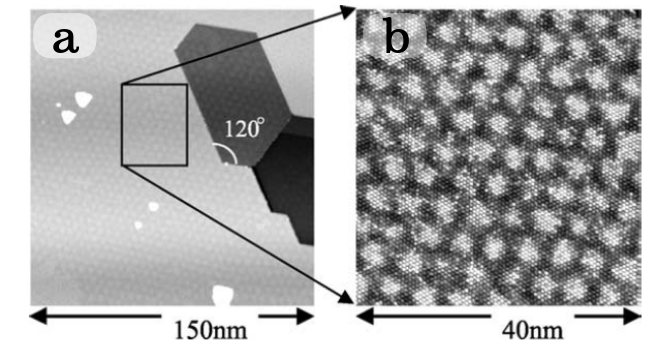
\includegraphics[width=1\linewidth]{poster_figures/Microscopy_label.png}
\end{minipage}
}

\headerbox{The Calculation Approach}{name=box_2, column=0, span=2, below=pics}{
\begin{minipage}{0.56\linewidth}
    \footnotesize{
        \par Density Functional Theory; generalized-gradient approximation (PBE) with D3(BJ) dispersion correction; VASP Code:
        \par Plane-wave basis sets (energy cut-off 450 eV);
        \par Special k-point sampling ($12\times12\times1$);
        \par Supercell (8 atoms for Graphene and BC\textsubscript{3} monolayers, 16 atoms for bilayer G-BC\textsubscript{3}); 
        \par Optimized lattice constant BC\textsubscript{3} , a = 5.165 Å (Exp: a = 5.2 Å) [6]
        \par Optimized lattice constant graphene, a = 4.936 Å  (or 2.468 Å for the unit cell)
        \par G-BC\textsubscript{3} heterostructure uses same lattice constant as BC\textsubscript{3} G under 5\% strain;
        \vspace{5pt}\par [6] H. Tanaka solid state communications 136 22-25 (2005)
    }\end{minipage}
    \hspace{1pt}\begin{minipage}{0.42\linewidth}
        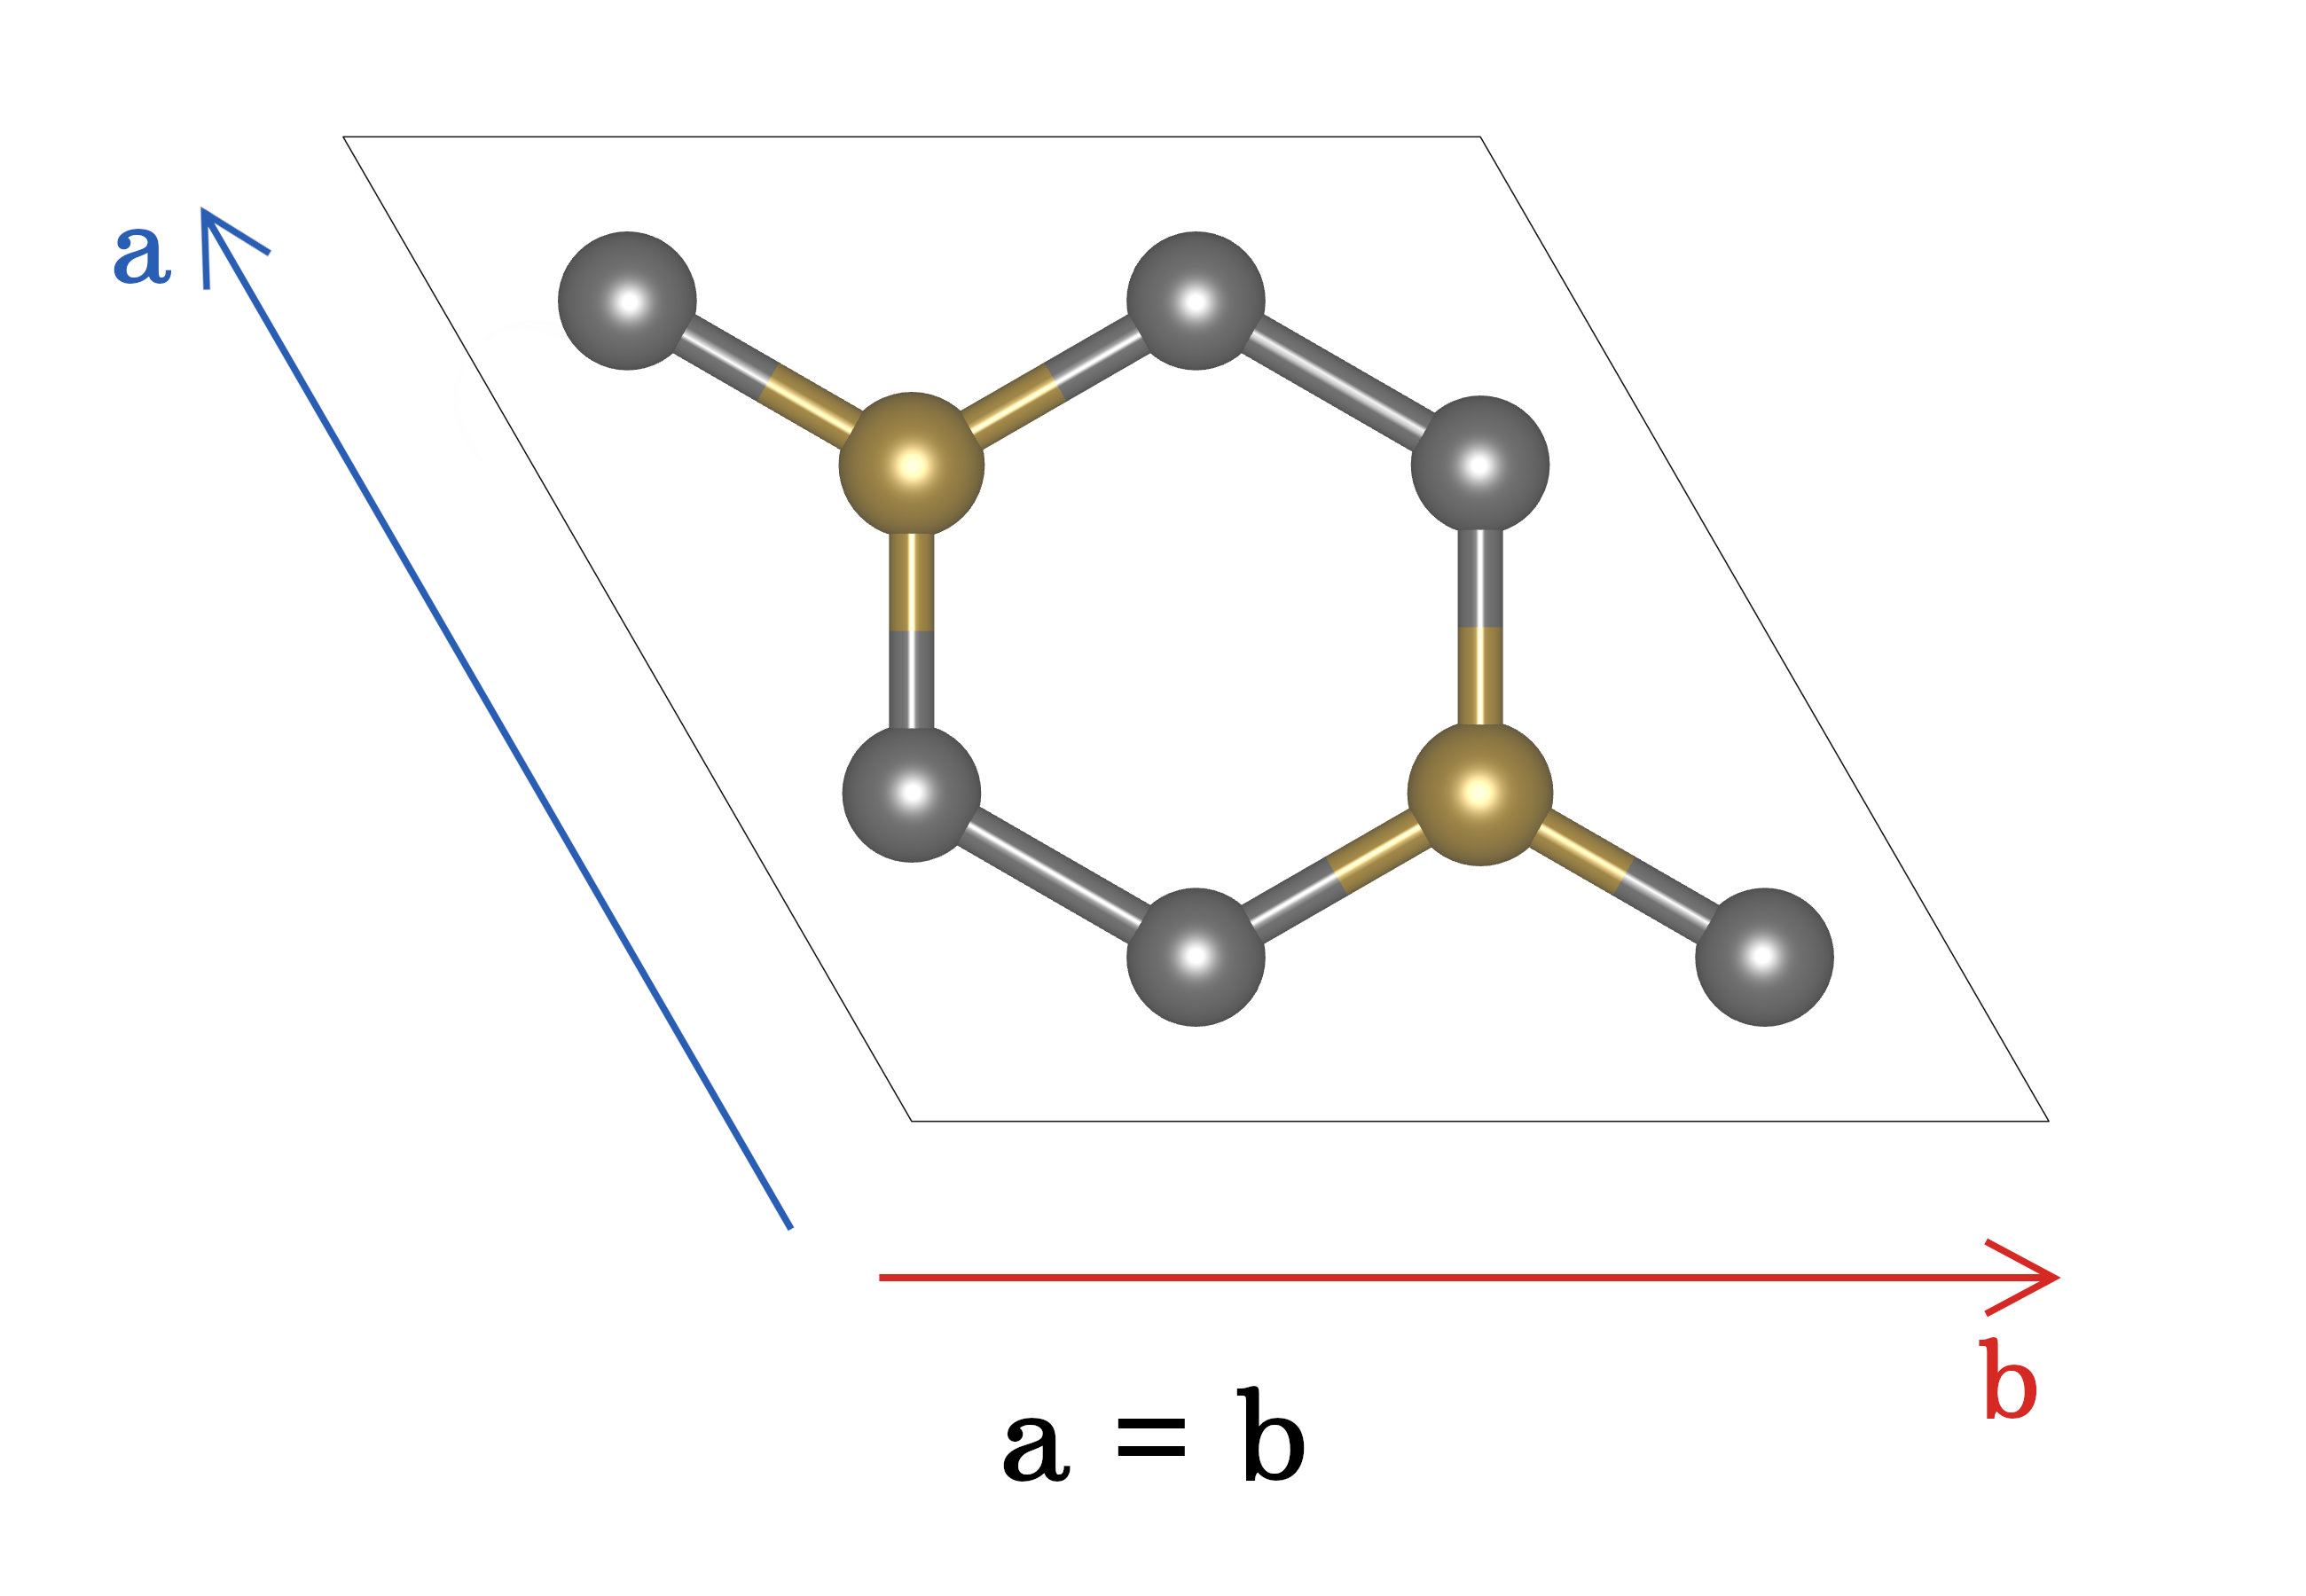
\includegraphics[width=1\linewidth]{poster_figures/BC3_cell_label.png}
        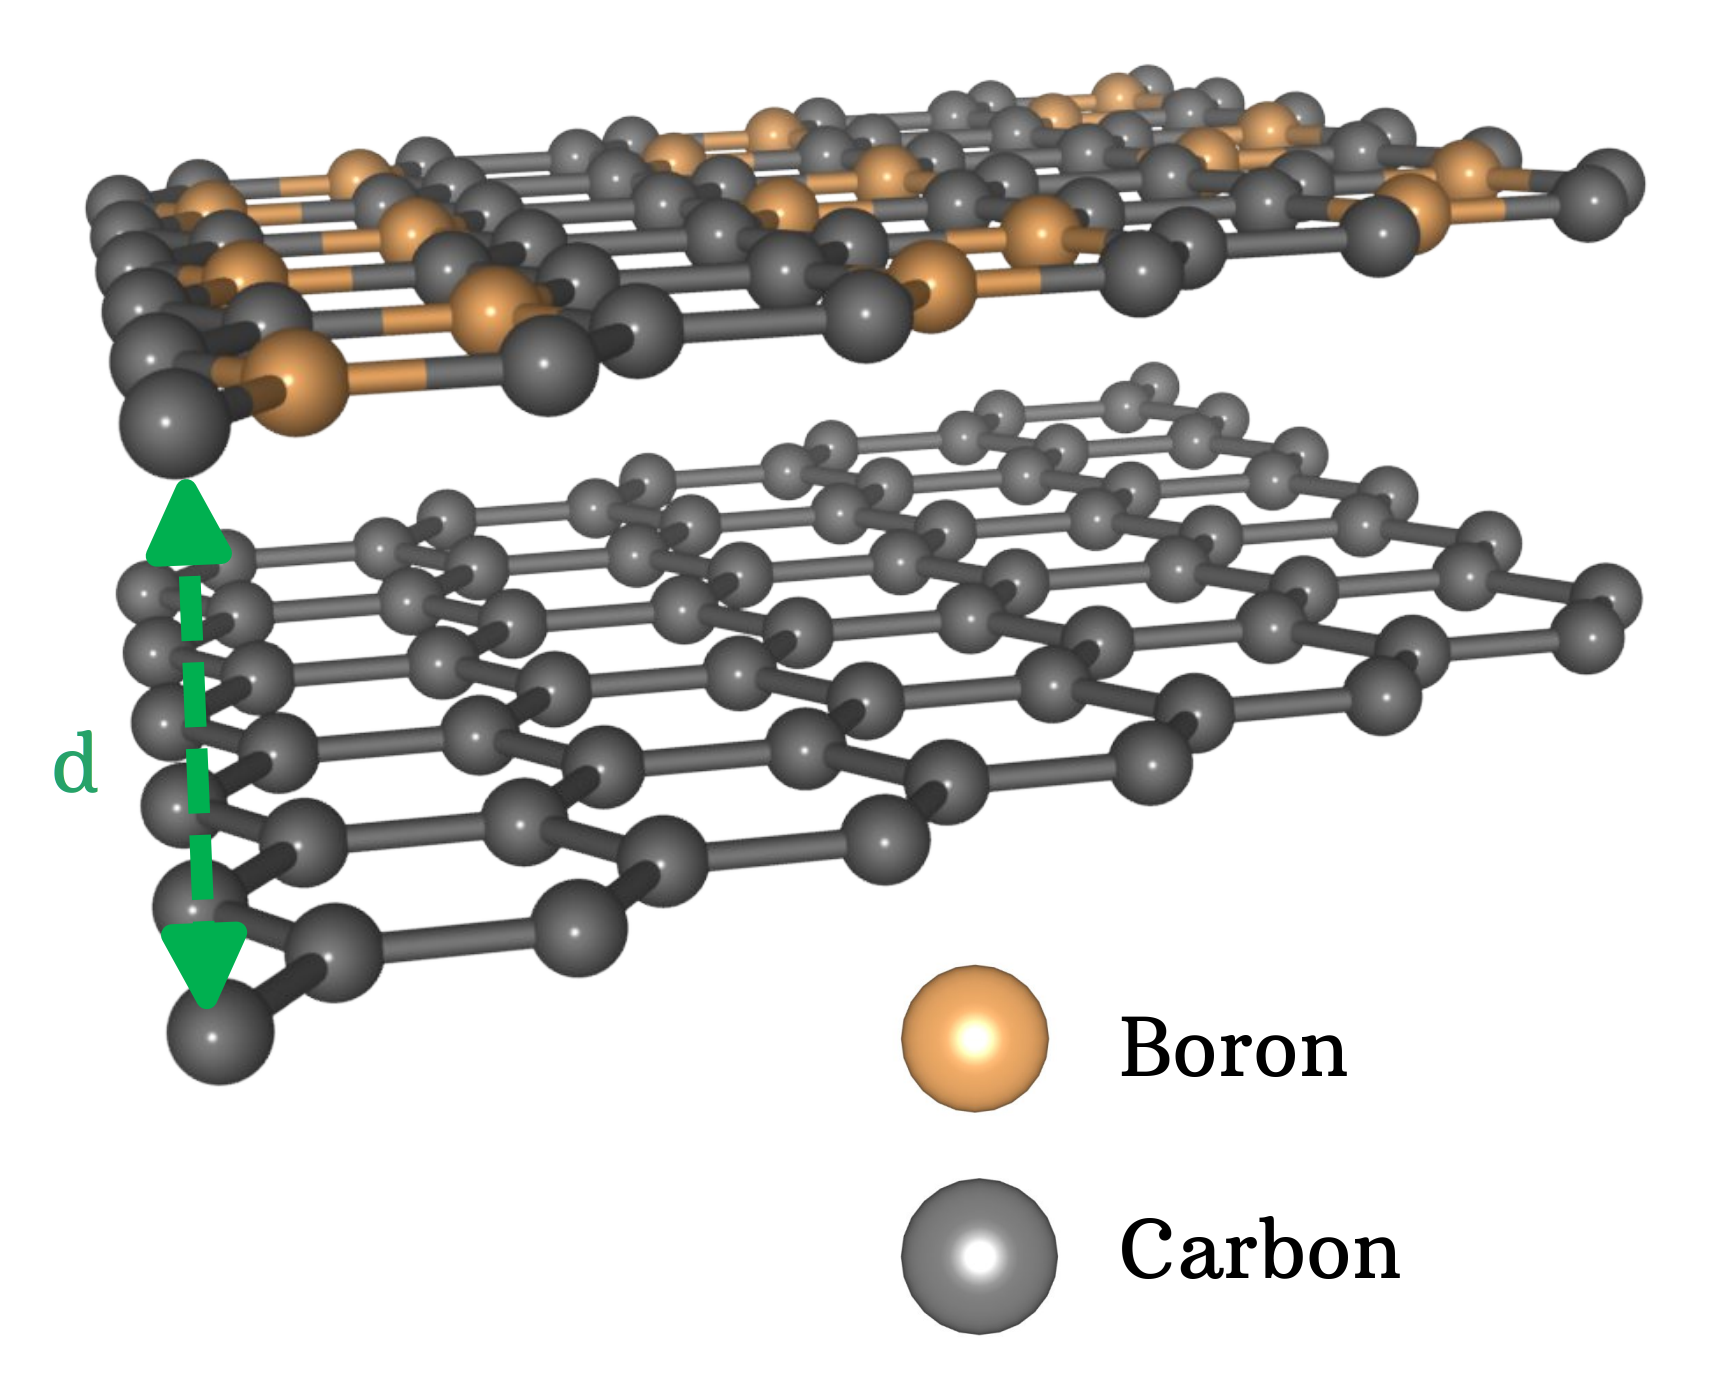
\includegraphics[width=1\linewidth]{poster_figures/Graphene-BC3.png}
\end{minipage}
}

\headerbox{Binding Energy: G-BC\textsubscript{3} heterostructure}{name=box_3, column=0, span=2, below=box_2}{
$$ E_\mathrm{b} = E_\mathrm{G-BC_3} - E_\mathrm{Graphene} - E_\mathrm{BC_3} $$
\par Where $E_\mathrm{b}$ is the binding energy;
\par $E_\mathrm{G-BC_3}$ is the energy of the bilayer Graphene-BC\textsubscript{3} system;
\par $E_\mathrm{Graphene}$ is the energy of monolayer graphene;
\par $E_\mathrm{BC_3}$  is the energy of monolayer BC\textsubscript{3}.
}

\headerbox{}{name=box_4, boxheaderheight=10pt, column=2, span=3}{

\begin{minipage}[t]{0.56\linewidth}\begin{center}
    \small\textbf{Favourable Bilayer Geometry}
    \par \textbf{Top} \qquad\qquad \textbf{Hollow} \qquad\qquad \textbf{Bridge}
    \par\includegraphics[width=0.32\linewidth]{poster_figures/G-BC3_top.png}
    \includegraphics[width=0.32\linewidth]{poster_figures/G-BC3_hollow.png}
    \includegraphics[width=0.32\linewidth]{poster_figures/G-BC3_bridge.png}
    \par
    \arrayrulecolor{white}\footnotesize
    \rowcolors[\hline]{2}{table_color_3}{table_color_2}
    \begin{tabular}{c|c|c|c}
    \rowcolor{table_color_1}\
        & Top & Hollow & Bridge \\
        Relative binding energy (eV) & 0.011 & 0 & 0.004 \\
        Interlayer distance (Å) & 3.467 & 3.431 & 3.435 \\
    \end{tabular}
\end{center}\end{minipage}
\begin{minipage}[t]{0.43\linewidth}\begin{center}
    \small\textbf{Graphene-BC\textsubscript{3} Interlayer Spacing}
    \par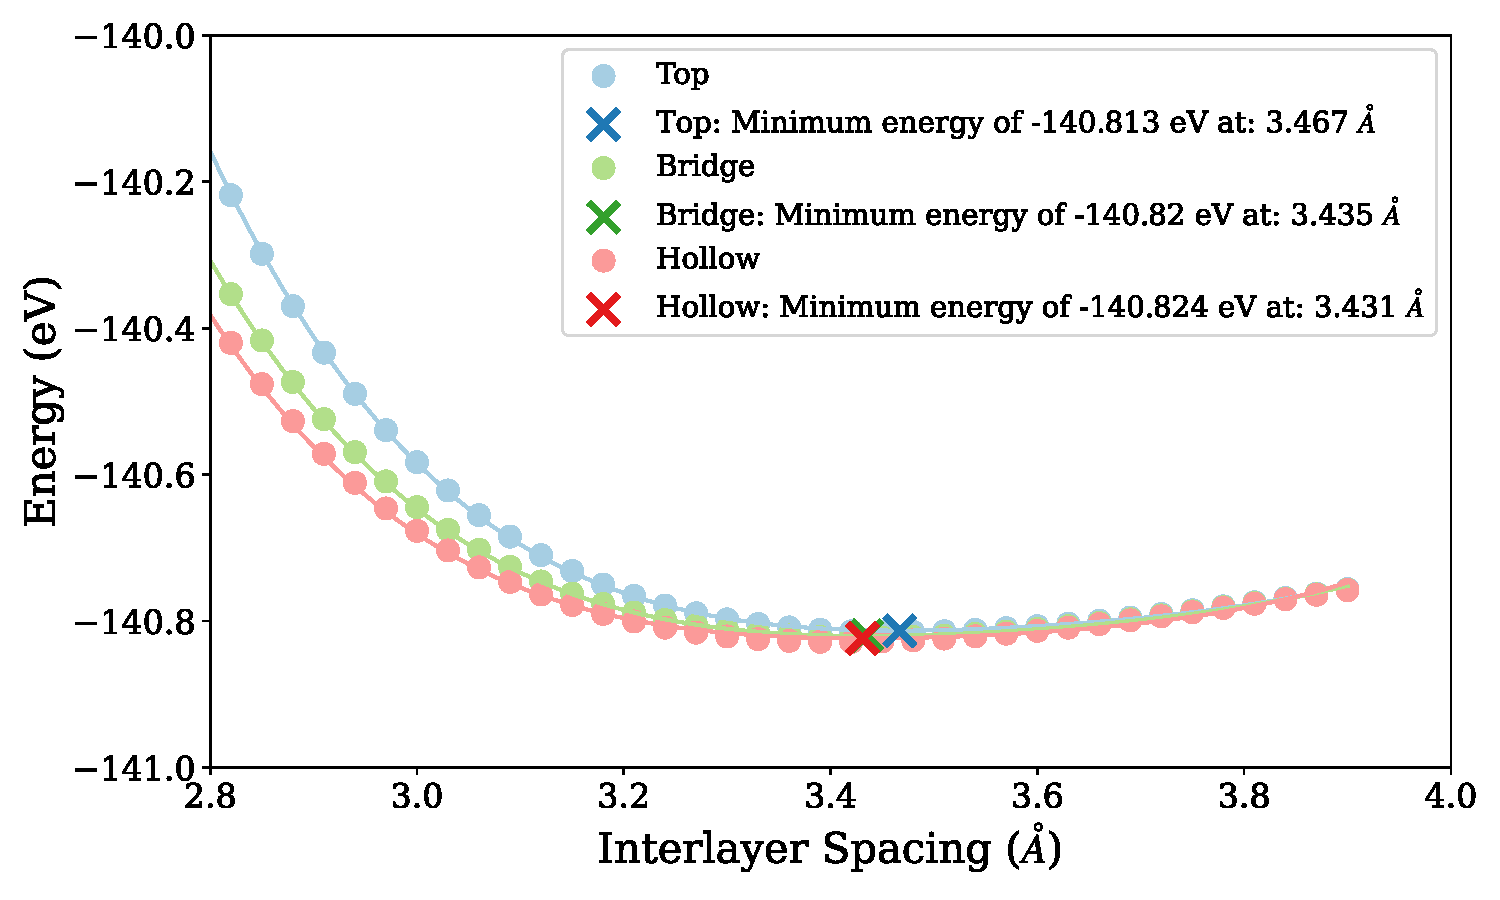
\includegraphics[width=0.8\linewidth]{poster_figures/G-BC3_interlayer_spacing.pdf}
\end{center}\end{minipage}

\begin{minipage}{1\linewidth}\begin{center}\footnotesize
    \begin{tcolorbox}[colback=table_color_2, colframe=table_color_2, rounded corners, boxsep=2pt, left=0pt, right=0pt, top=0pt, bottom=0pt]
        \par $\bullet$ The relative bilayer top, hollow and bridge sites are tested by fixing the graphene layer and translating the BC\textsubscript{3} layer.
        \par $\bullet$ The hollow site shows the most favorable binding energy and is the preferred Graphene-BC\textsubscript{3} configuration.
    \end{tcolorbox}
\end{center}\end{minipage}

\begin{center}\small\textbf{Graphene}\end{center}

\vspace{-5pt}\begin{minipage}[t]{0.72\linewidth}\begin{center}
    \small\textcolor{dark_blue}{\textbf{Electronic Properties}}
\end{center}\end{minipage}
\begin{minipage}[t]{0.24\linewidth}\begin{center}
    \small\textcolor{dark_blue}{\textbf{Optical Properties}}
\end{center}\end{minipage}

\begin{minipage}[t]{1\linewidth}\begin{center}
    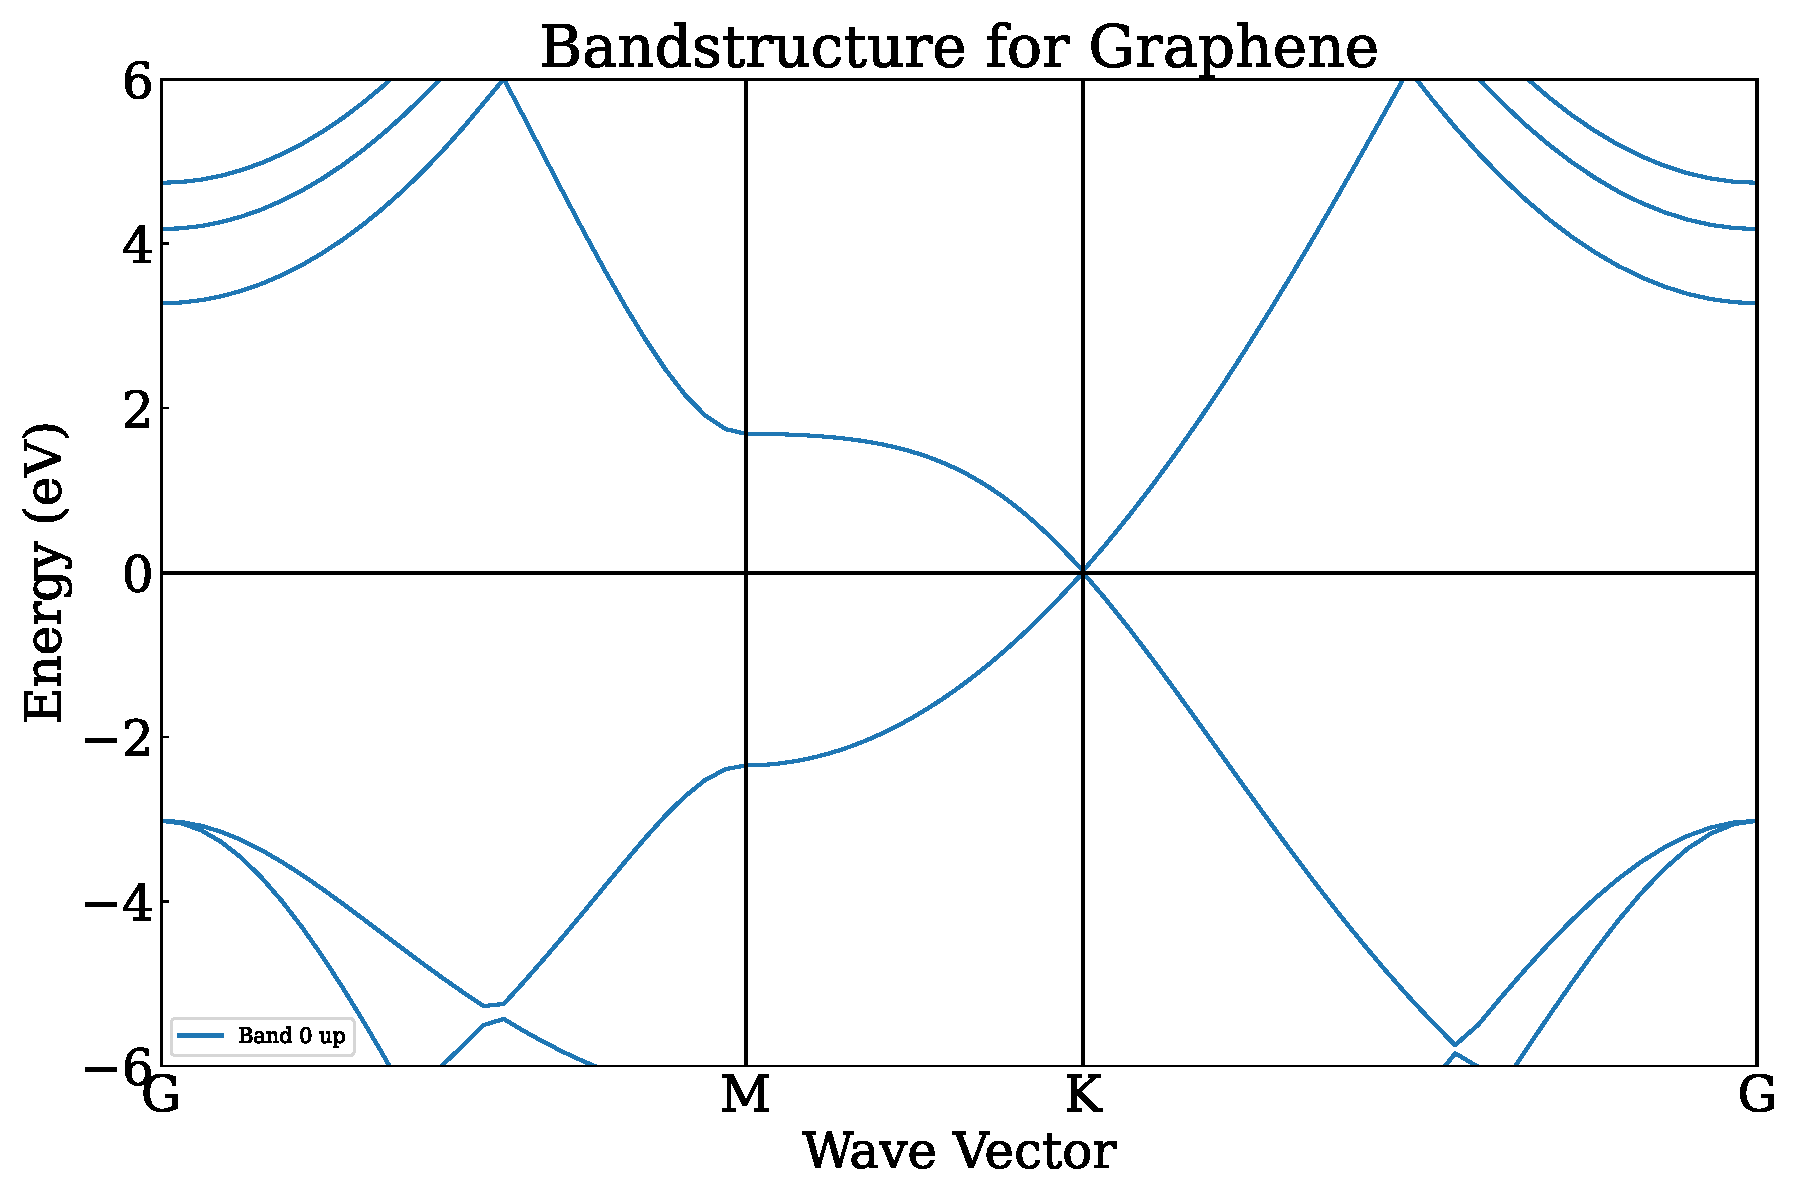
\includegraphics[width=0.30\linewidth]{poster_figures/G_BS.pdf}
    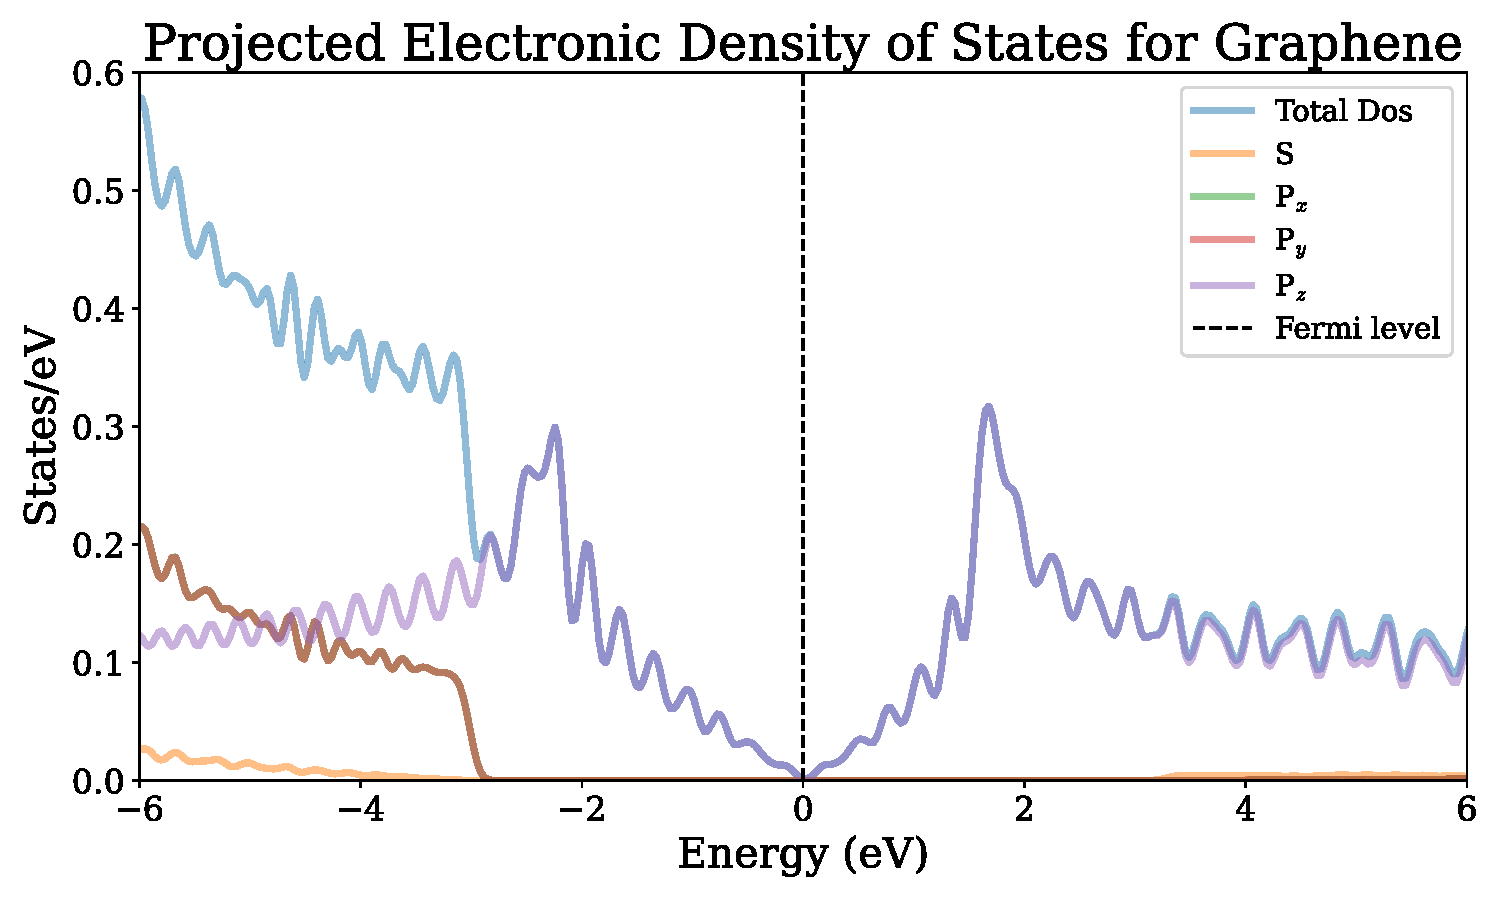
\includegraphics[width=0.30\linewidth]{poster_figures/G_PDOS.pdf}
    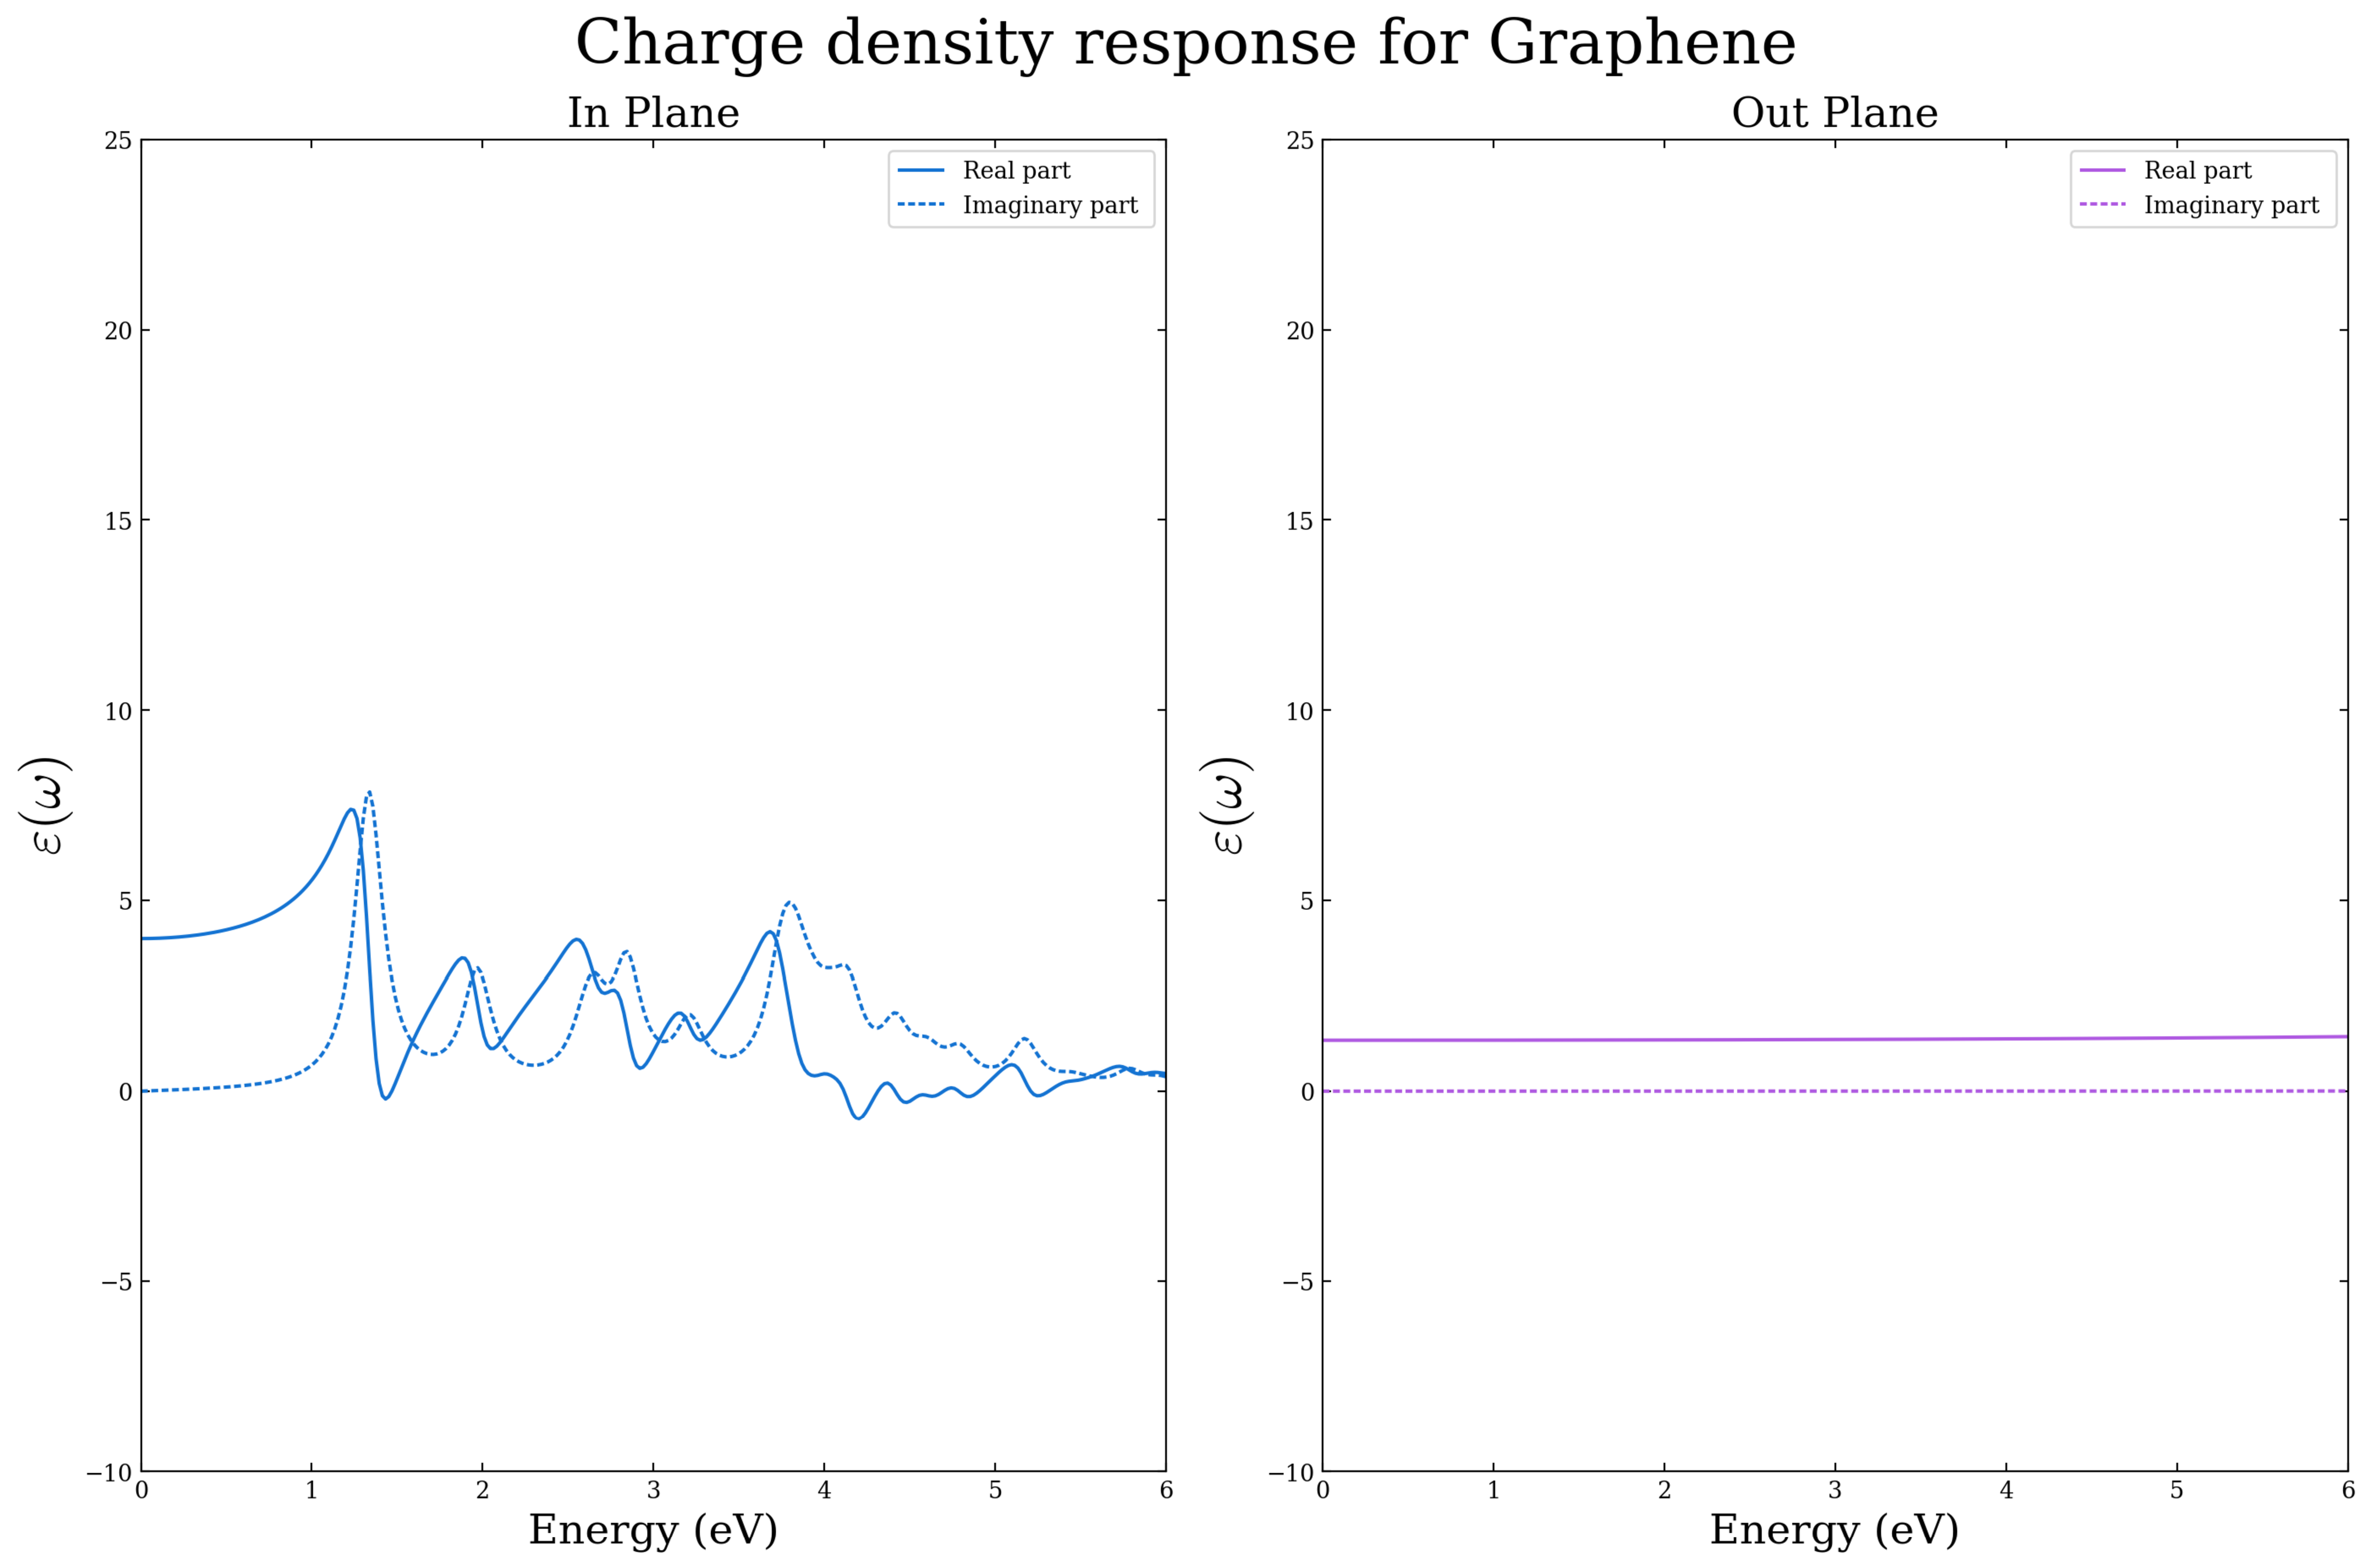
\includegraphics[width=0.30\linewidth]{poster_figures/G_opt.pdf}
\end{center}\end{minipage}

\vspace{0pt}\begin{minipage}{1\linewidth}\begin{center}\footnotesize
    \begin{tcolorbox}[colback=table_color_2, colframe=table_color_2, rounded corners, boxsep=2pt, left=0pt, right=0pt, top=0pt, bottom=0pt]
        \par $\bullet$ Graphene's well-known semimetallic behavior is shown by the Dirac cone at the Fermi level (0 eV). 
        \par $\bullet$ Broad in-plane dielectric response from the NIR and across the visible spectrum.
    \end{tcolorbox}
\end{center}\end{minipage}

\begin{center}\small\textbf{BC\textsubscript{3}}\end{center}

\begin{minipage}[t]{1\linewidth}\begin{center}
    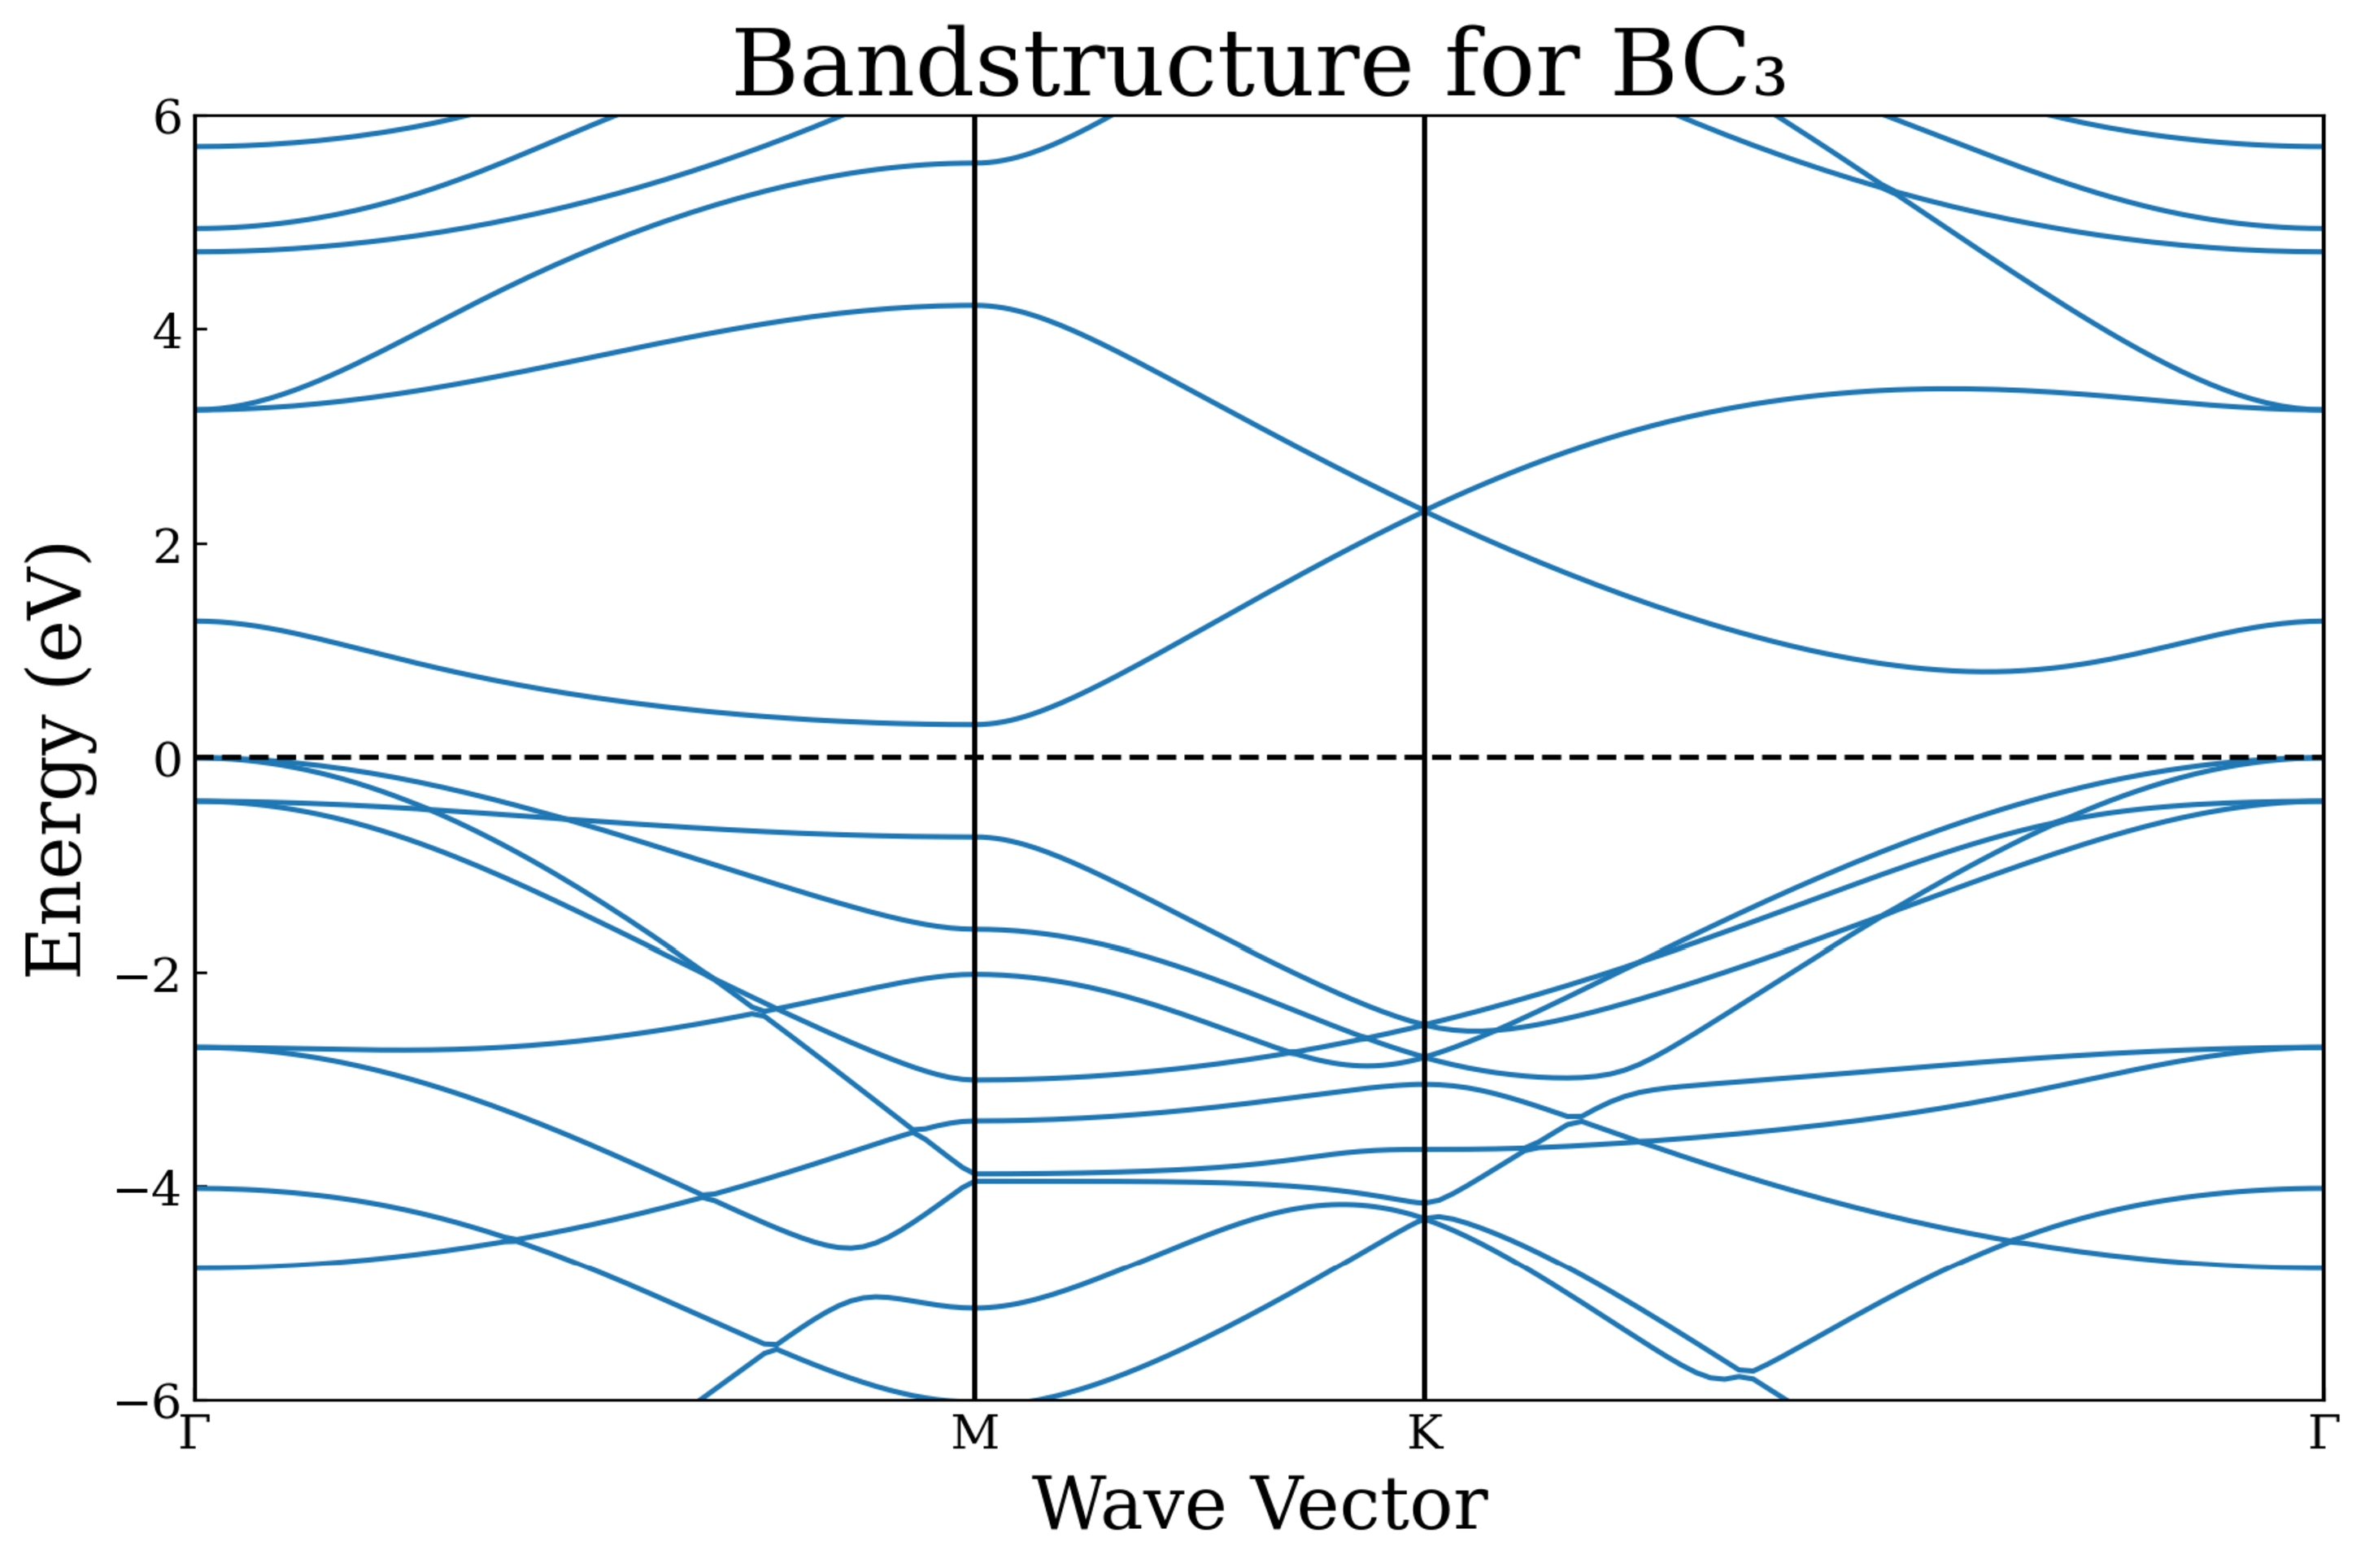
\includegraphics[width=0.30\linewidth]{poster_figures/BC3_BS.pdf}
    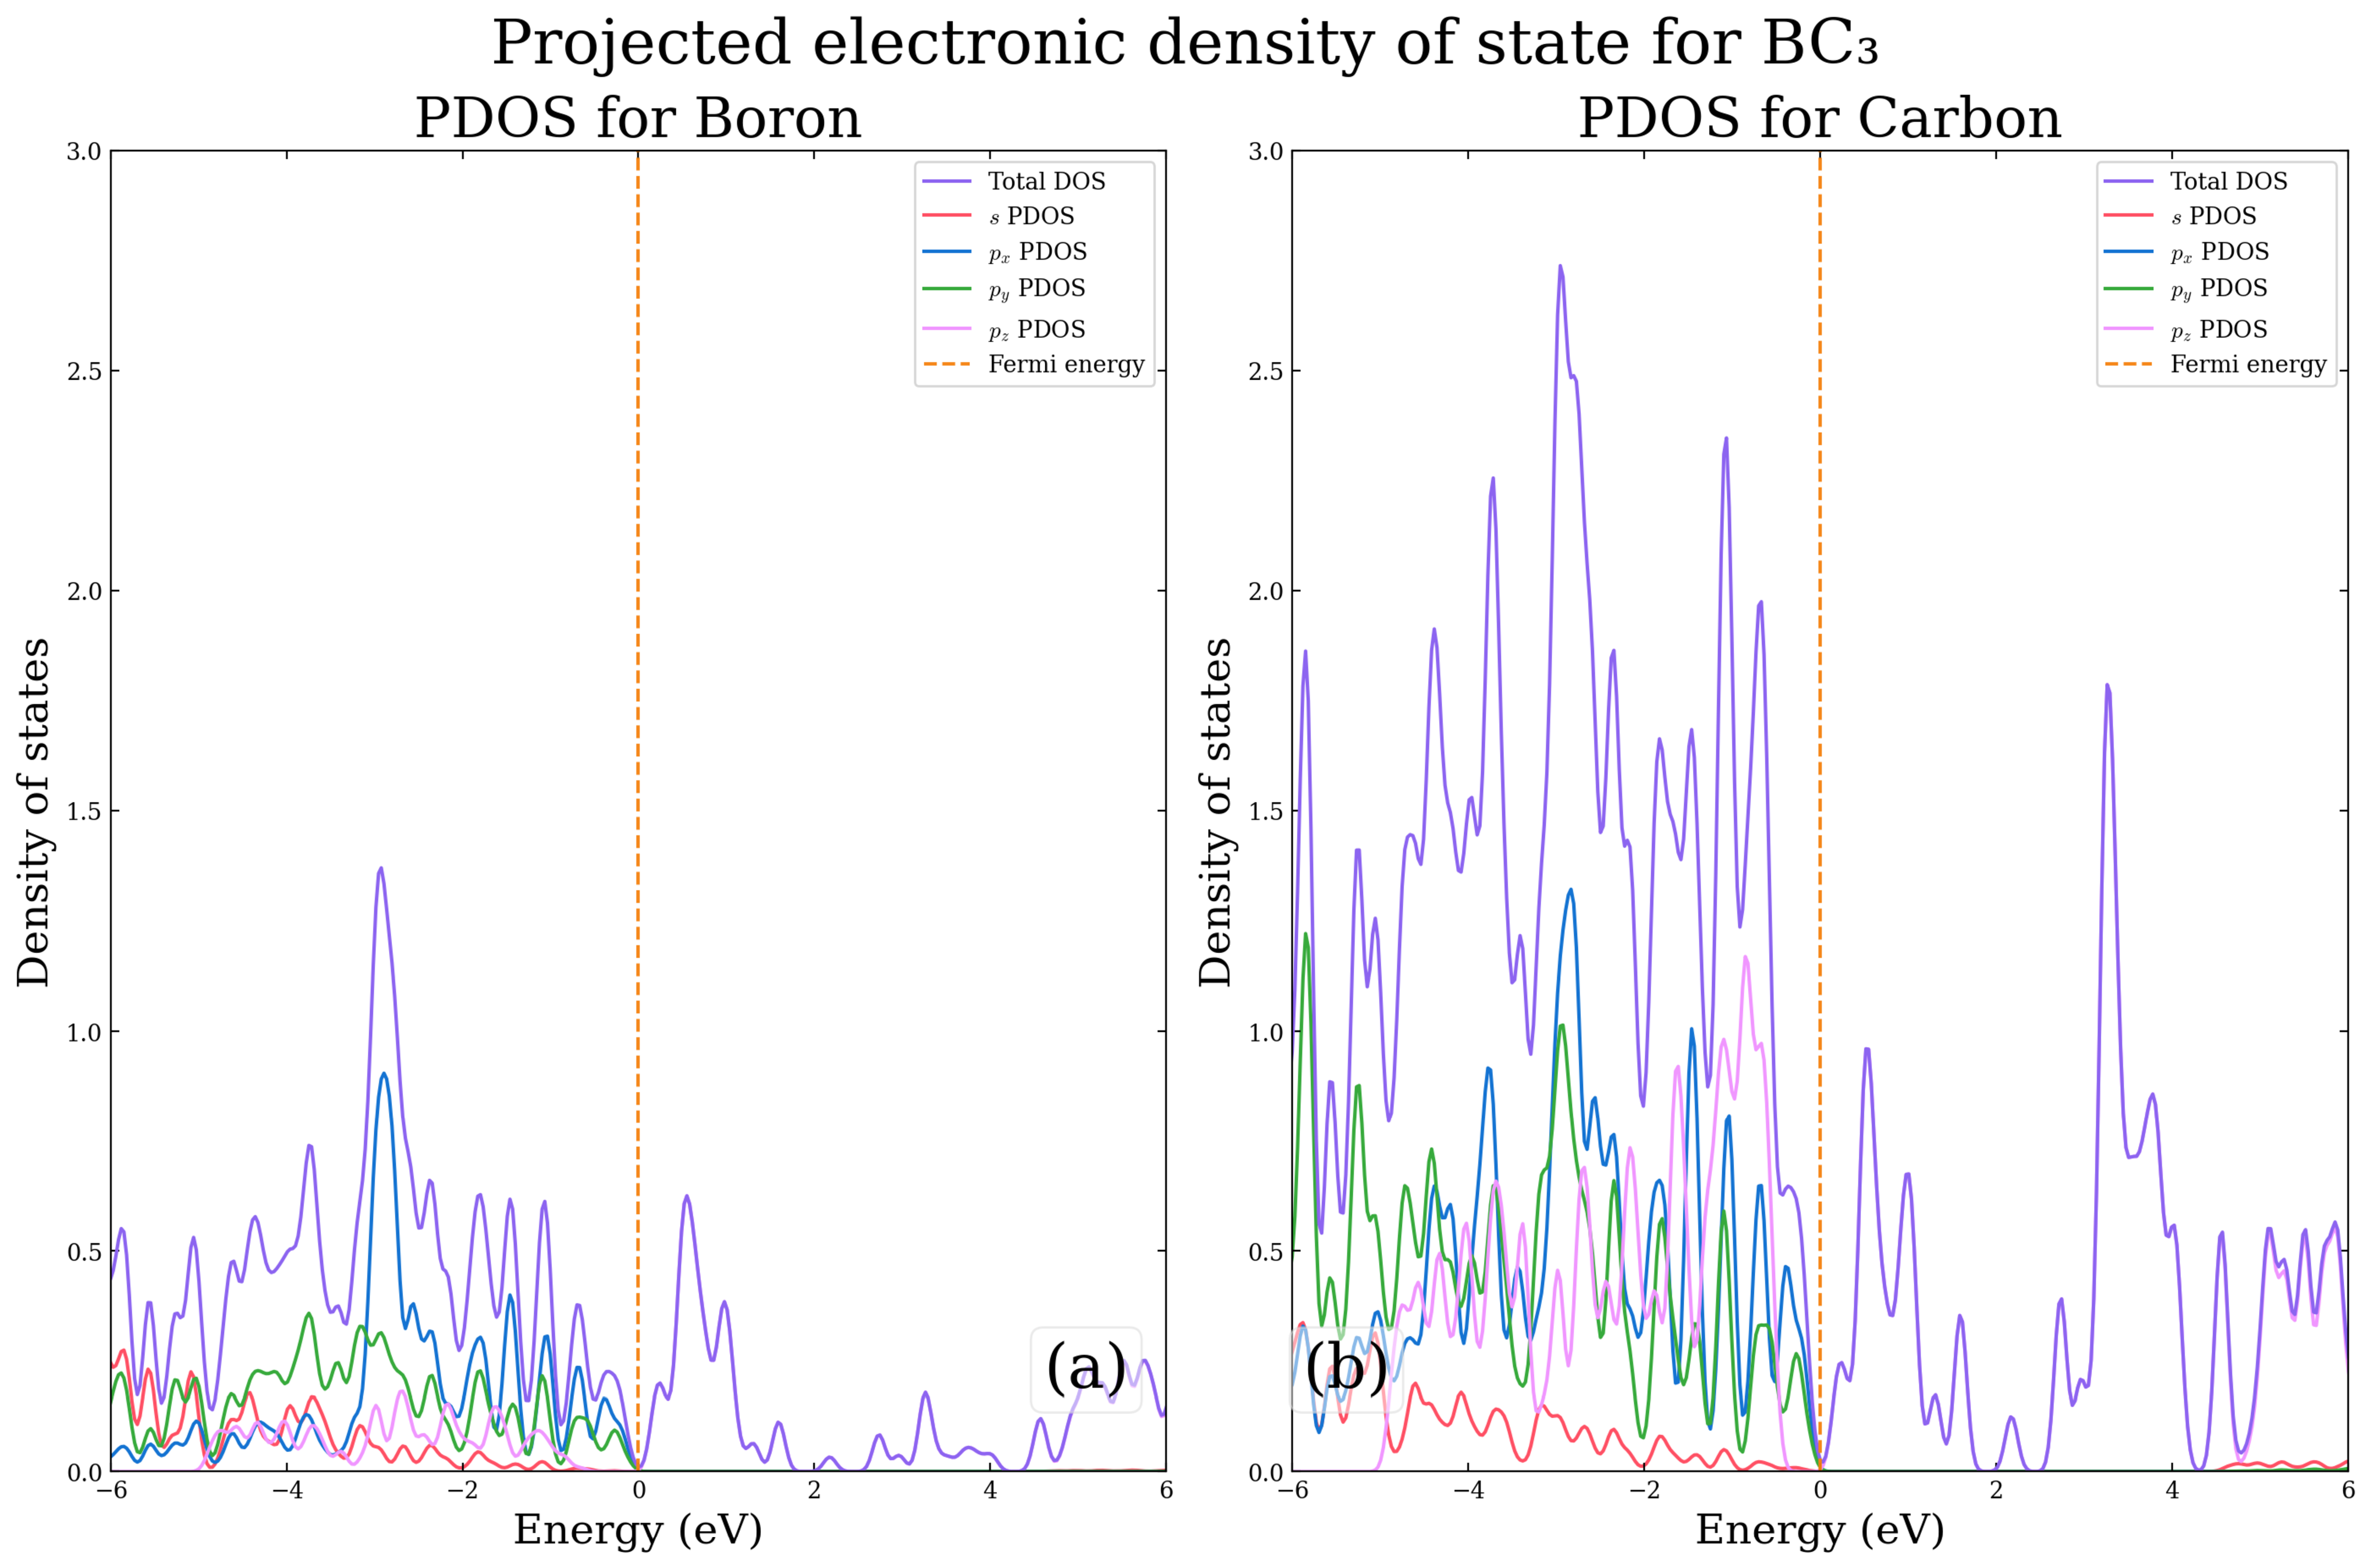
\includegraphics[width=0.30\linewidth]{poster_figures/BC3_PDOS.pdf}
    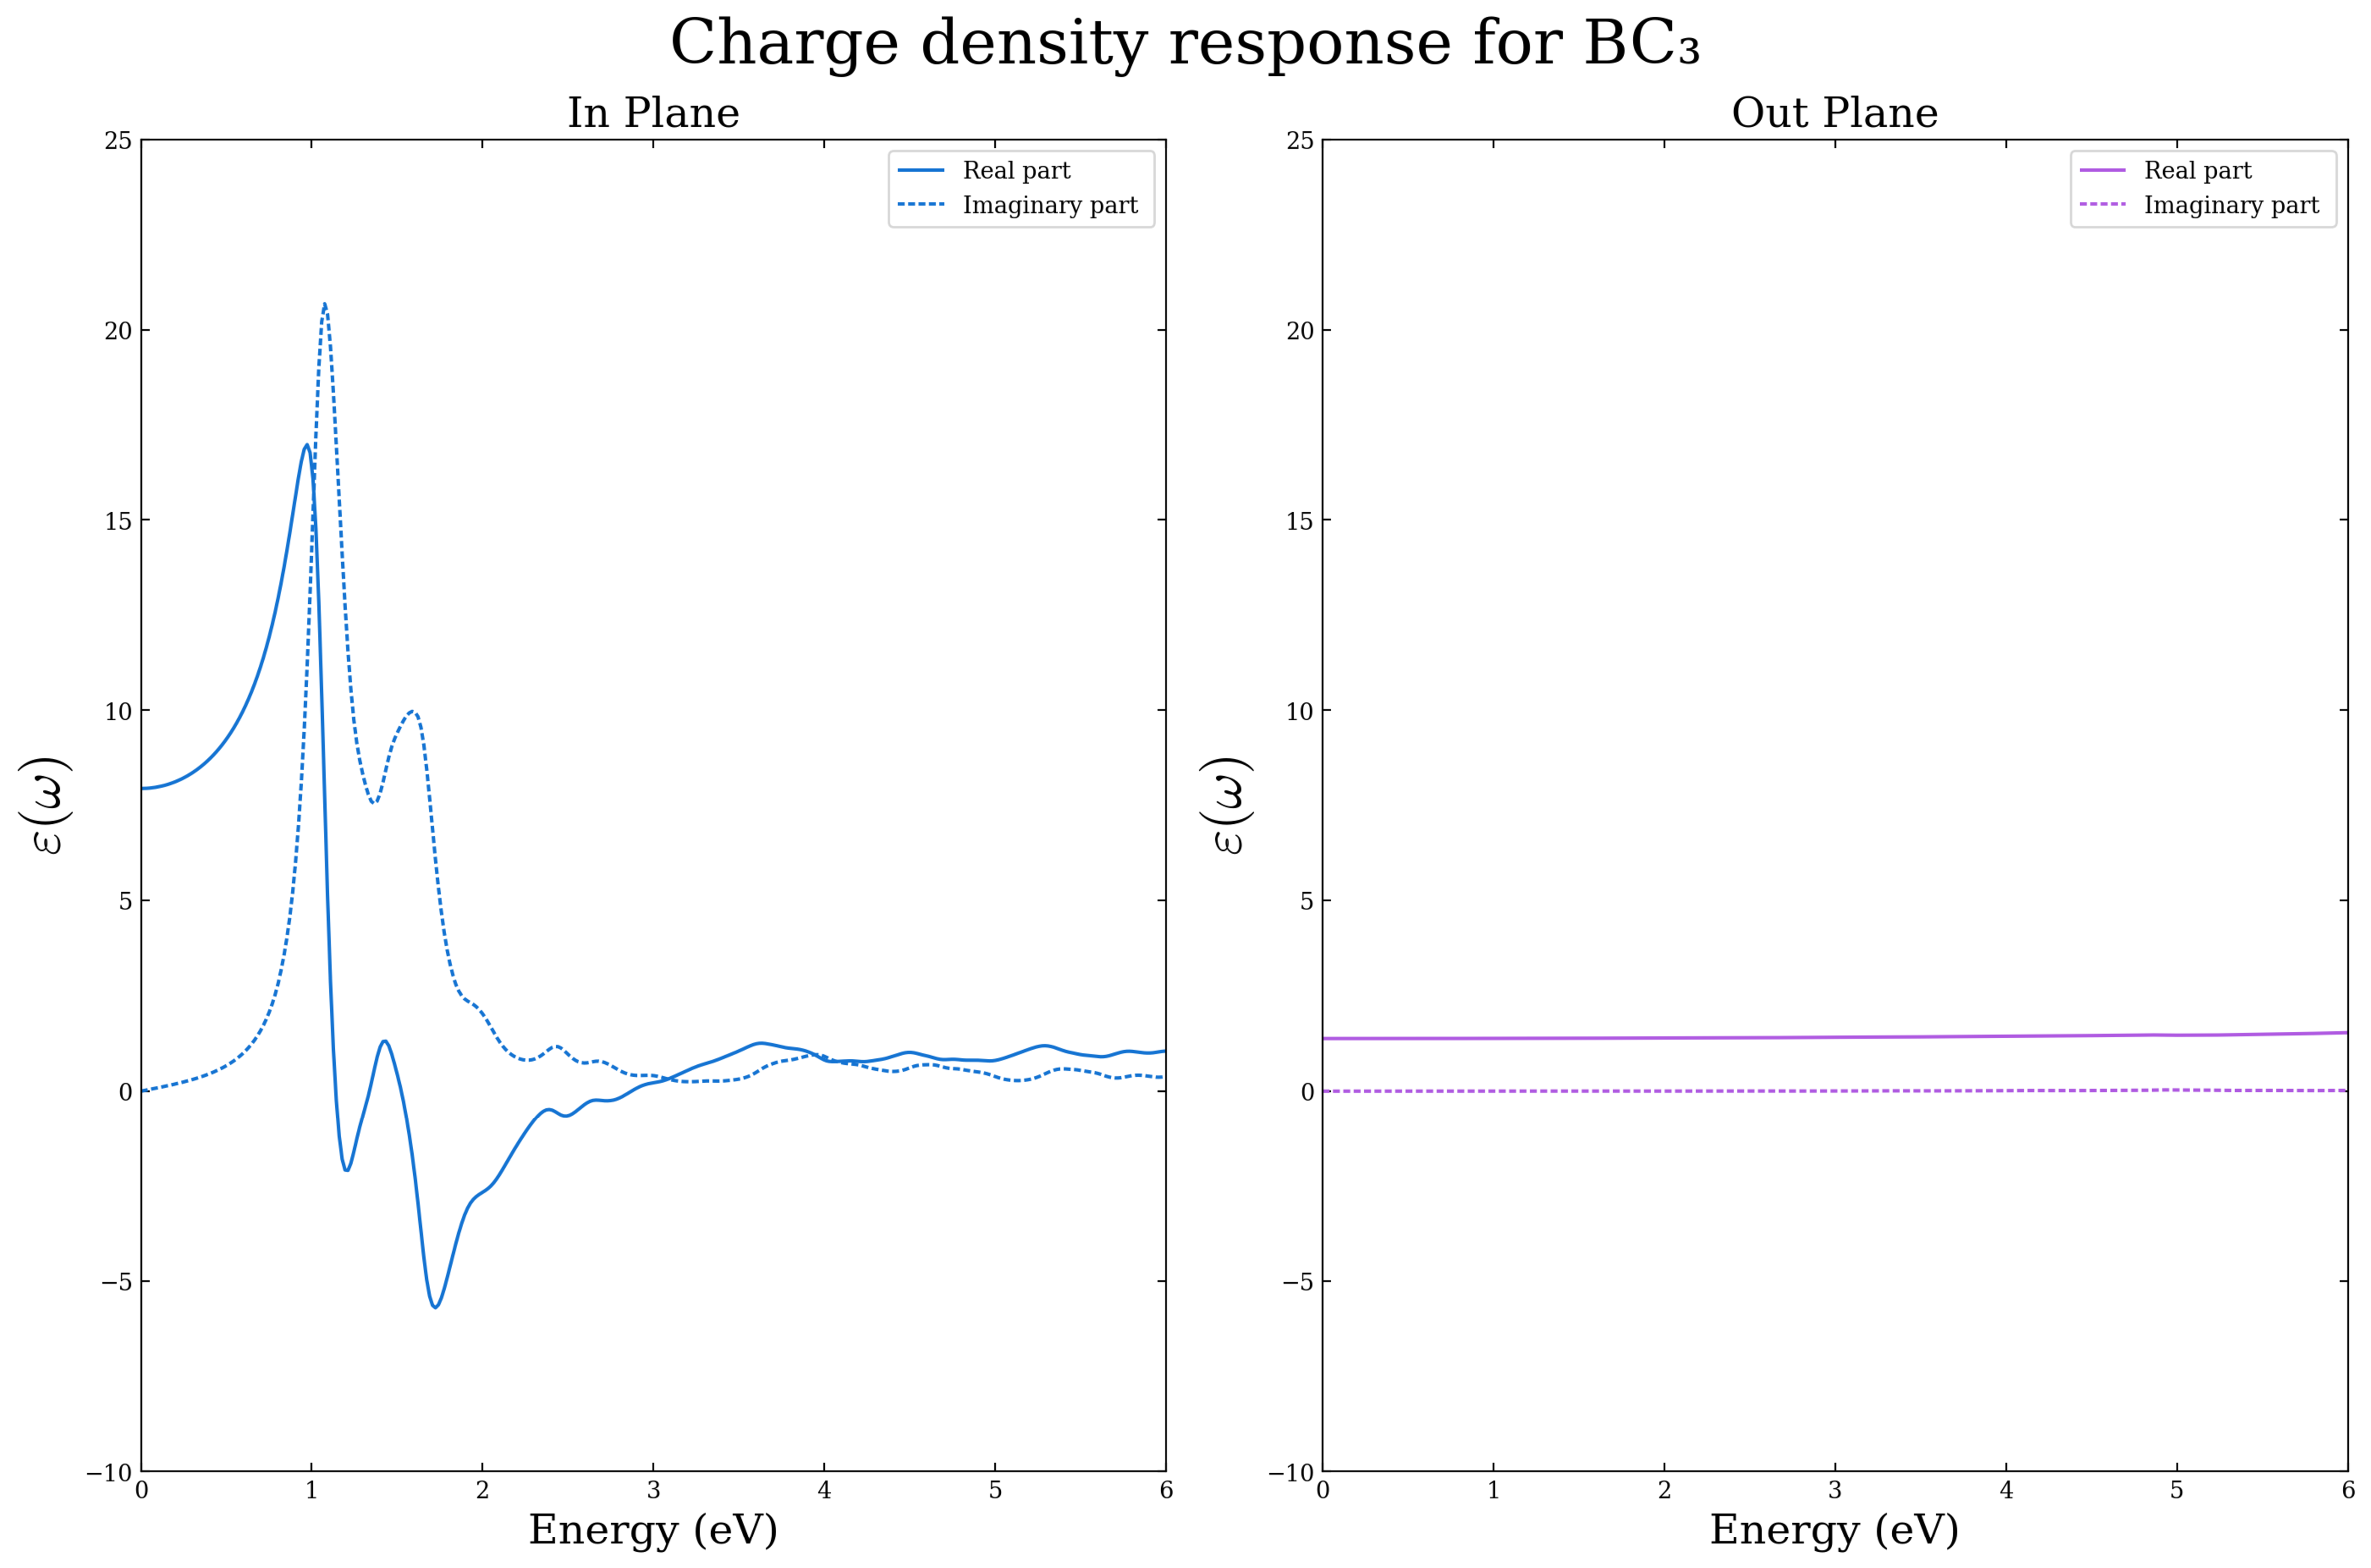
\includegraphics[width=0.30\linewidth]{poster_figures/BC3_opt.pdf}
\end{center}\end{minipage}

\vspace{0pt}\begin{minipage}{1\linewidth}\begin{center}\footnotesize
    \begin{tcolorbox}[colback=table_color_2, colframe=table_color_2, rounded corners, boxsep=2pt, left=0pt, right=0pt, top=0pt, bottom=0pt]
        \par $\bullet$ Unlike graphene, BC\textsubscript{3} shows semiconducting behavior with a band-gap of 0.327 eV.
        \par $\bullet$ Relatively stronger in-plane dielectric response in the NIR and long wavelength visible range compared to Graphene.
    \end{tcolorbox}
\end{center}\end{minipage}

\begin{center}\small\textbf{Graphene-BC\textsubscript{3} heterostructure}\end{center}

\begin{minipage}[t]{1\linewidth}\begin{center}
    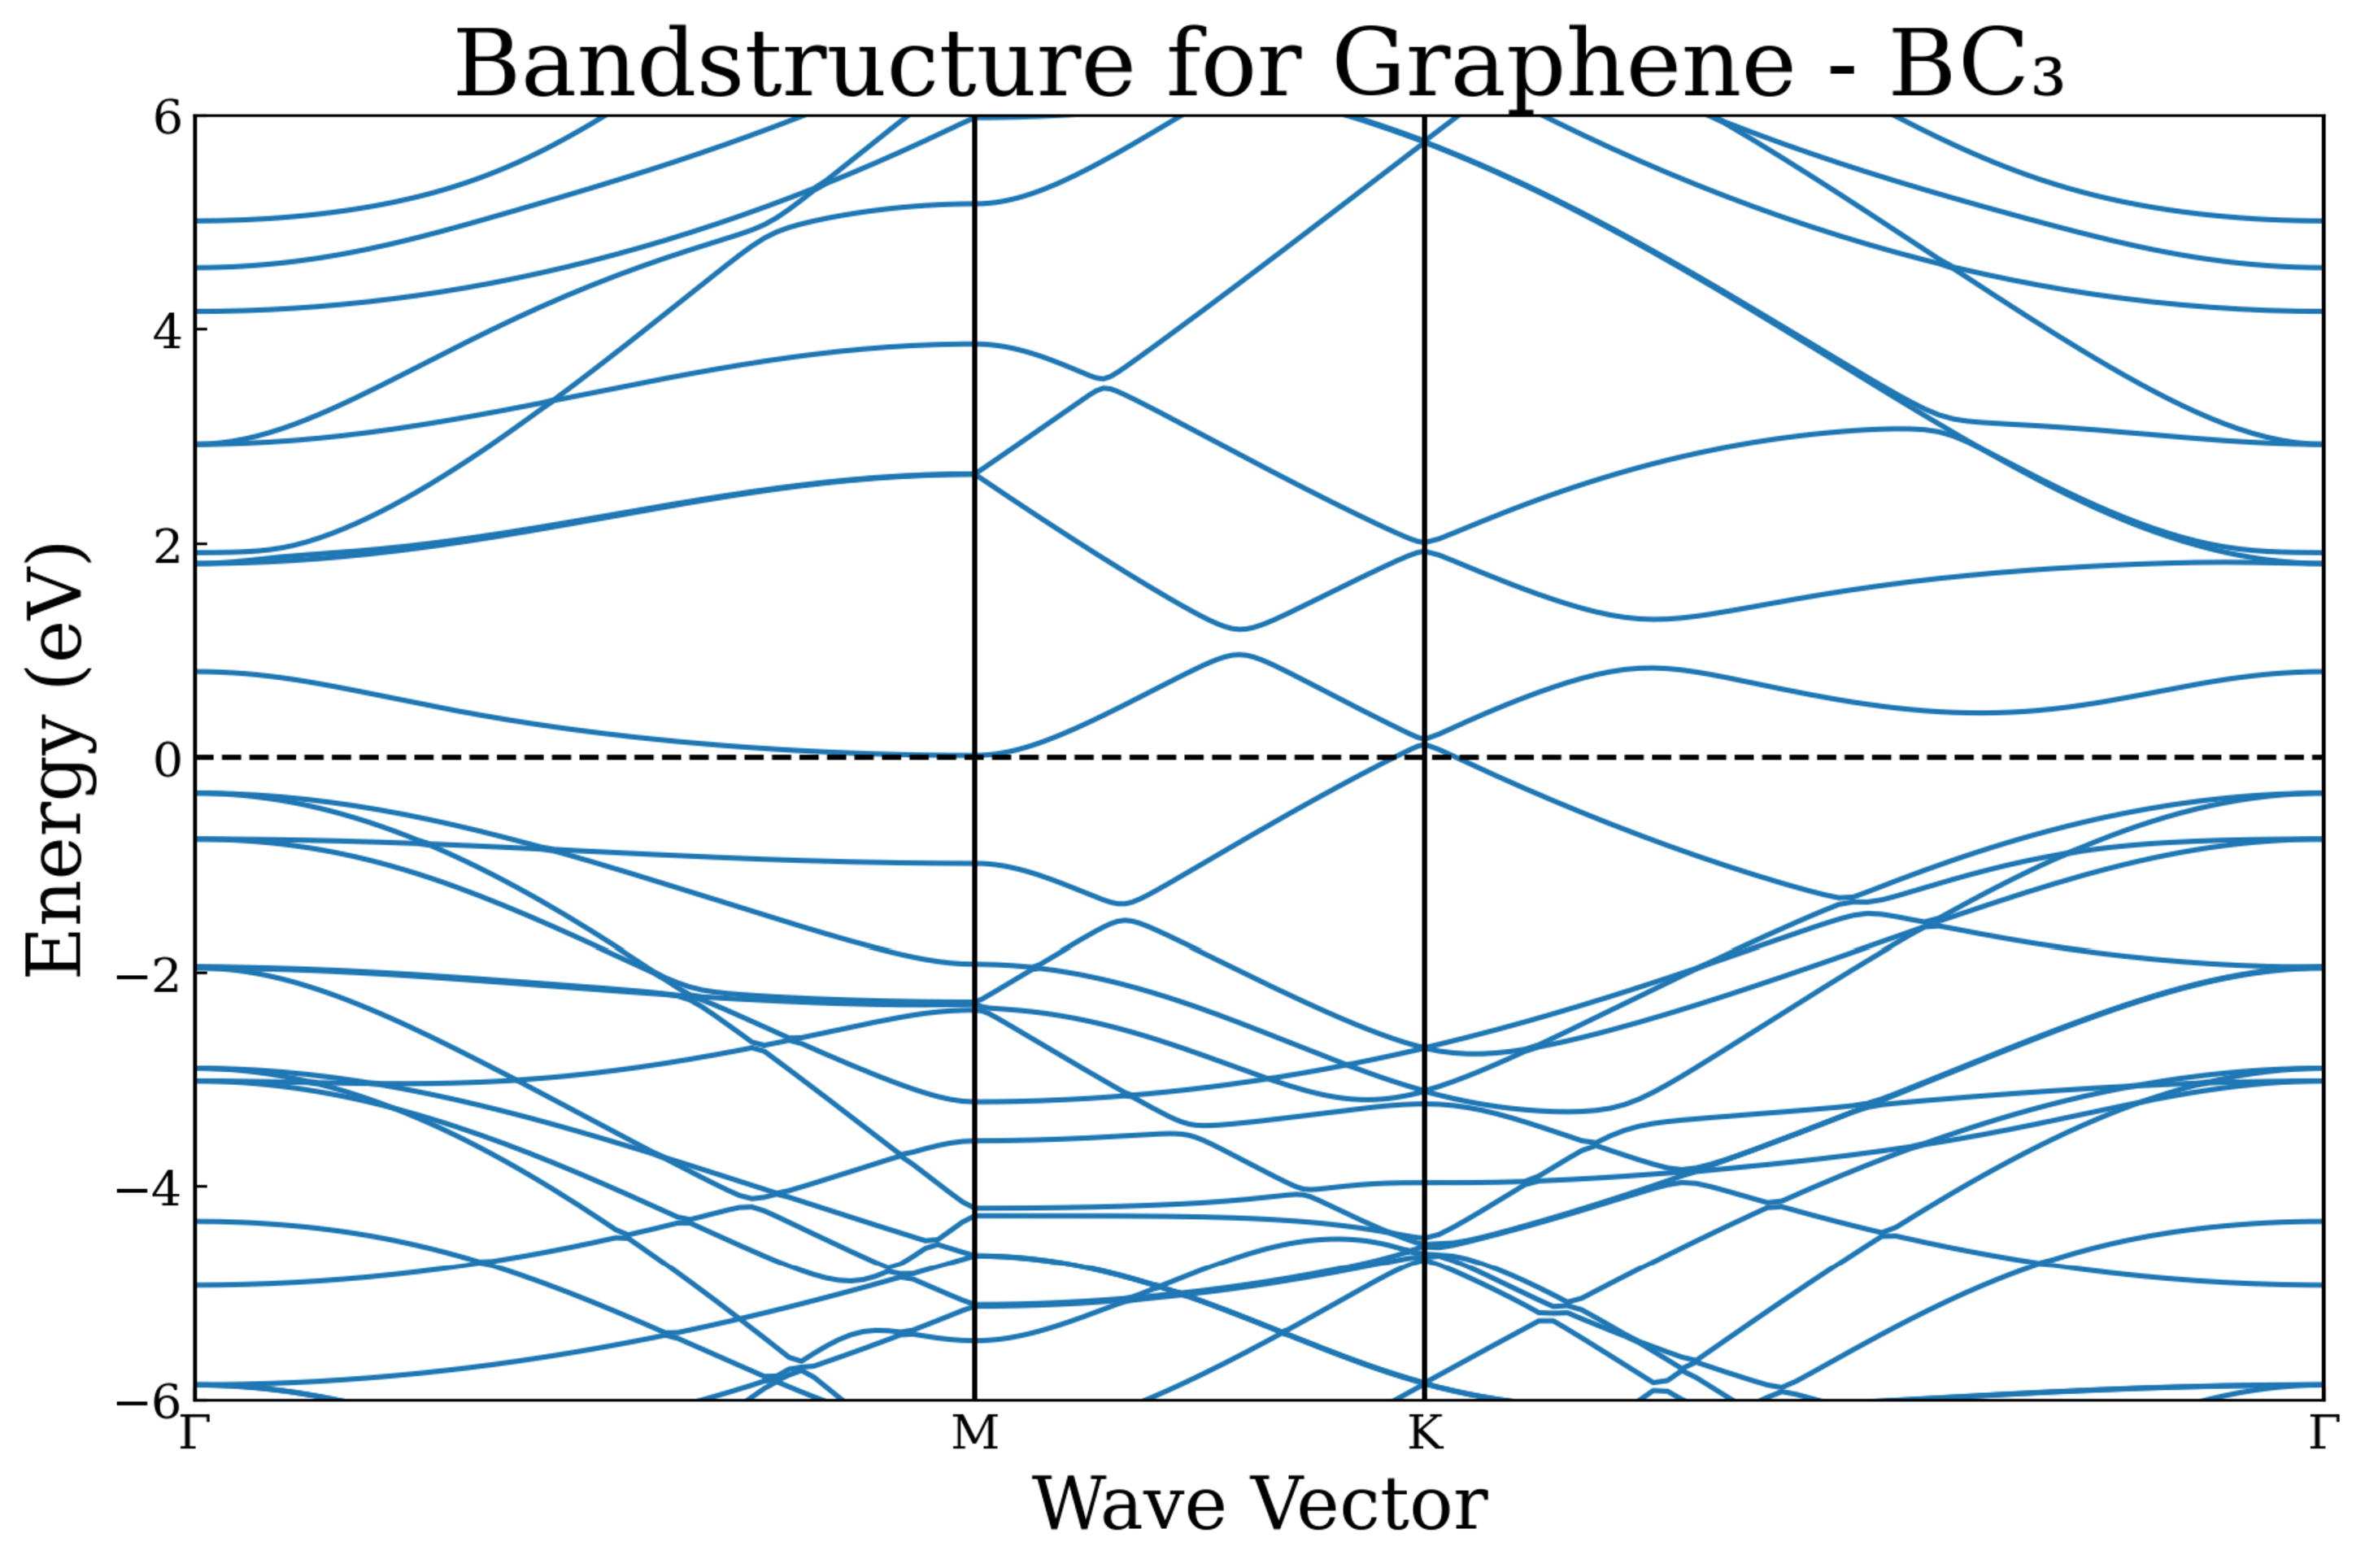
\includegraphics[width=0.30\linewidth]{poster_figures/G-BC3_BS.pdf}
    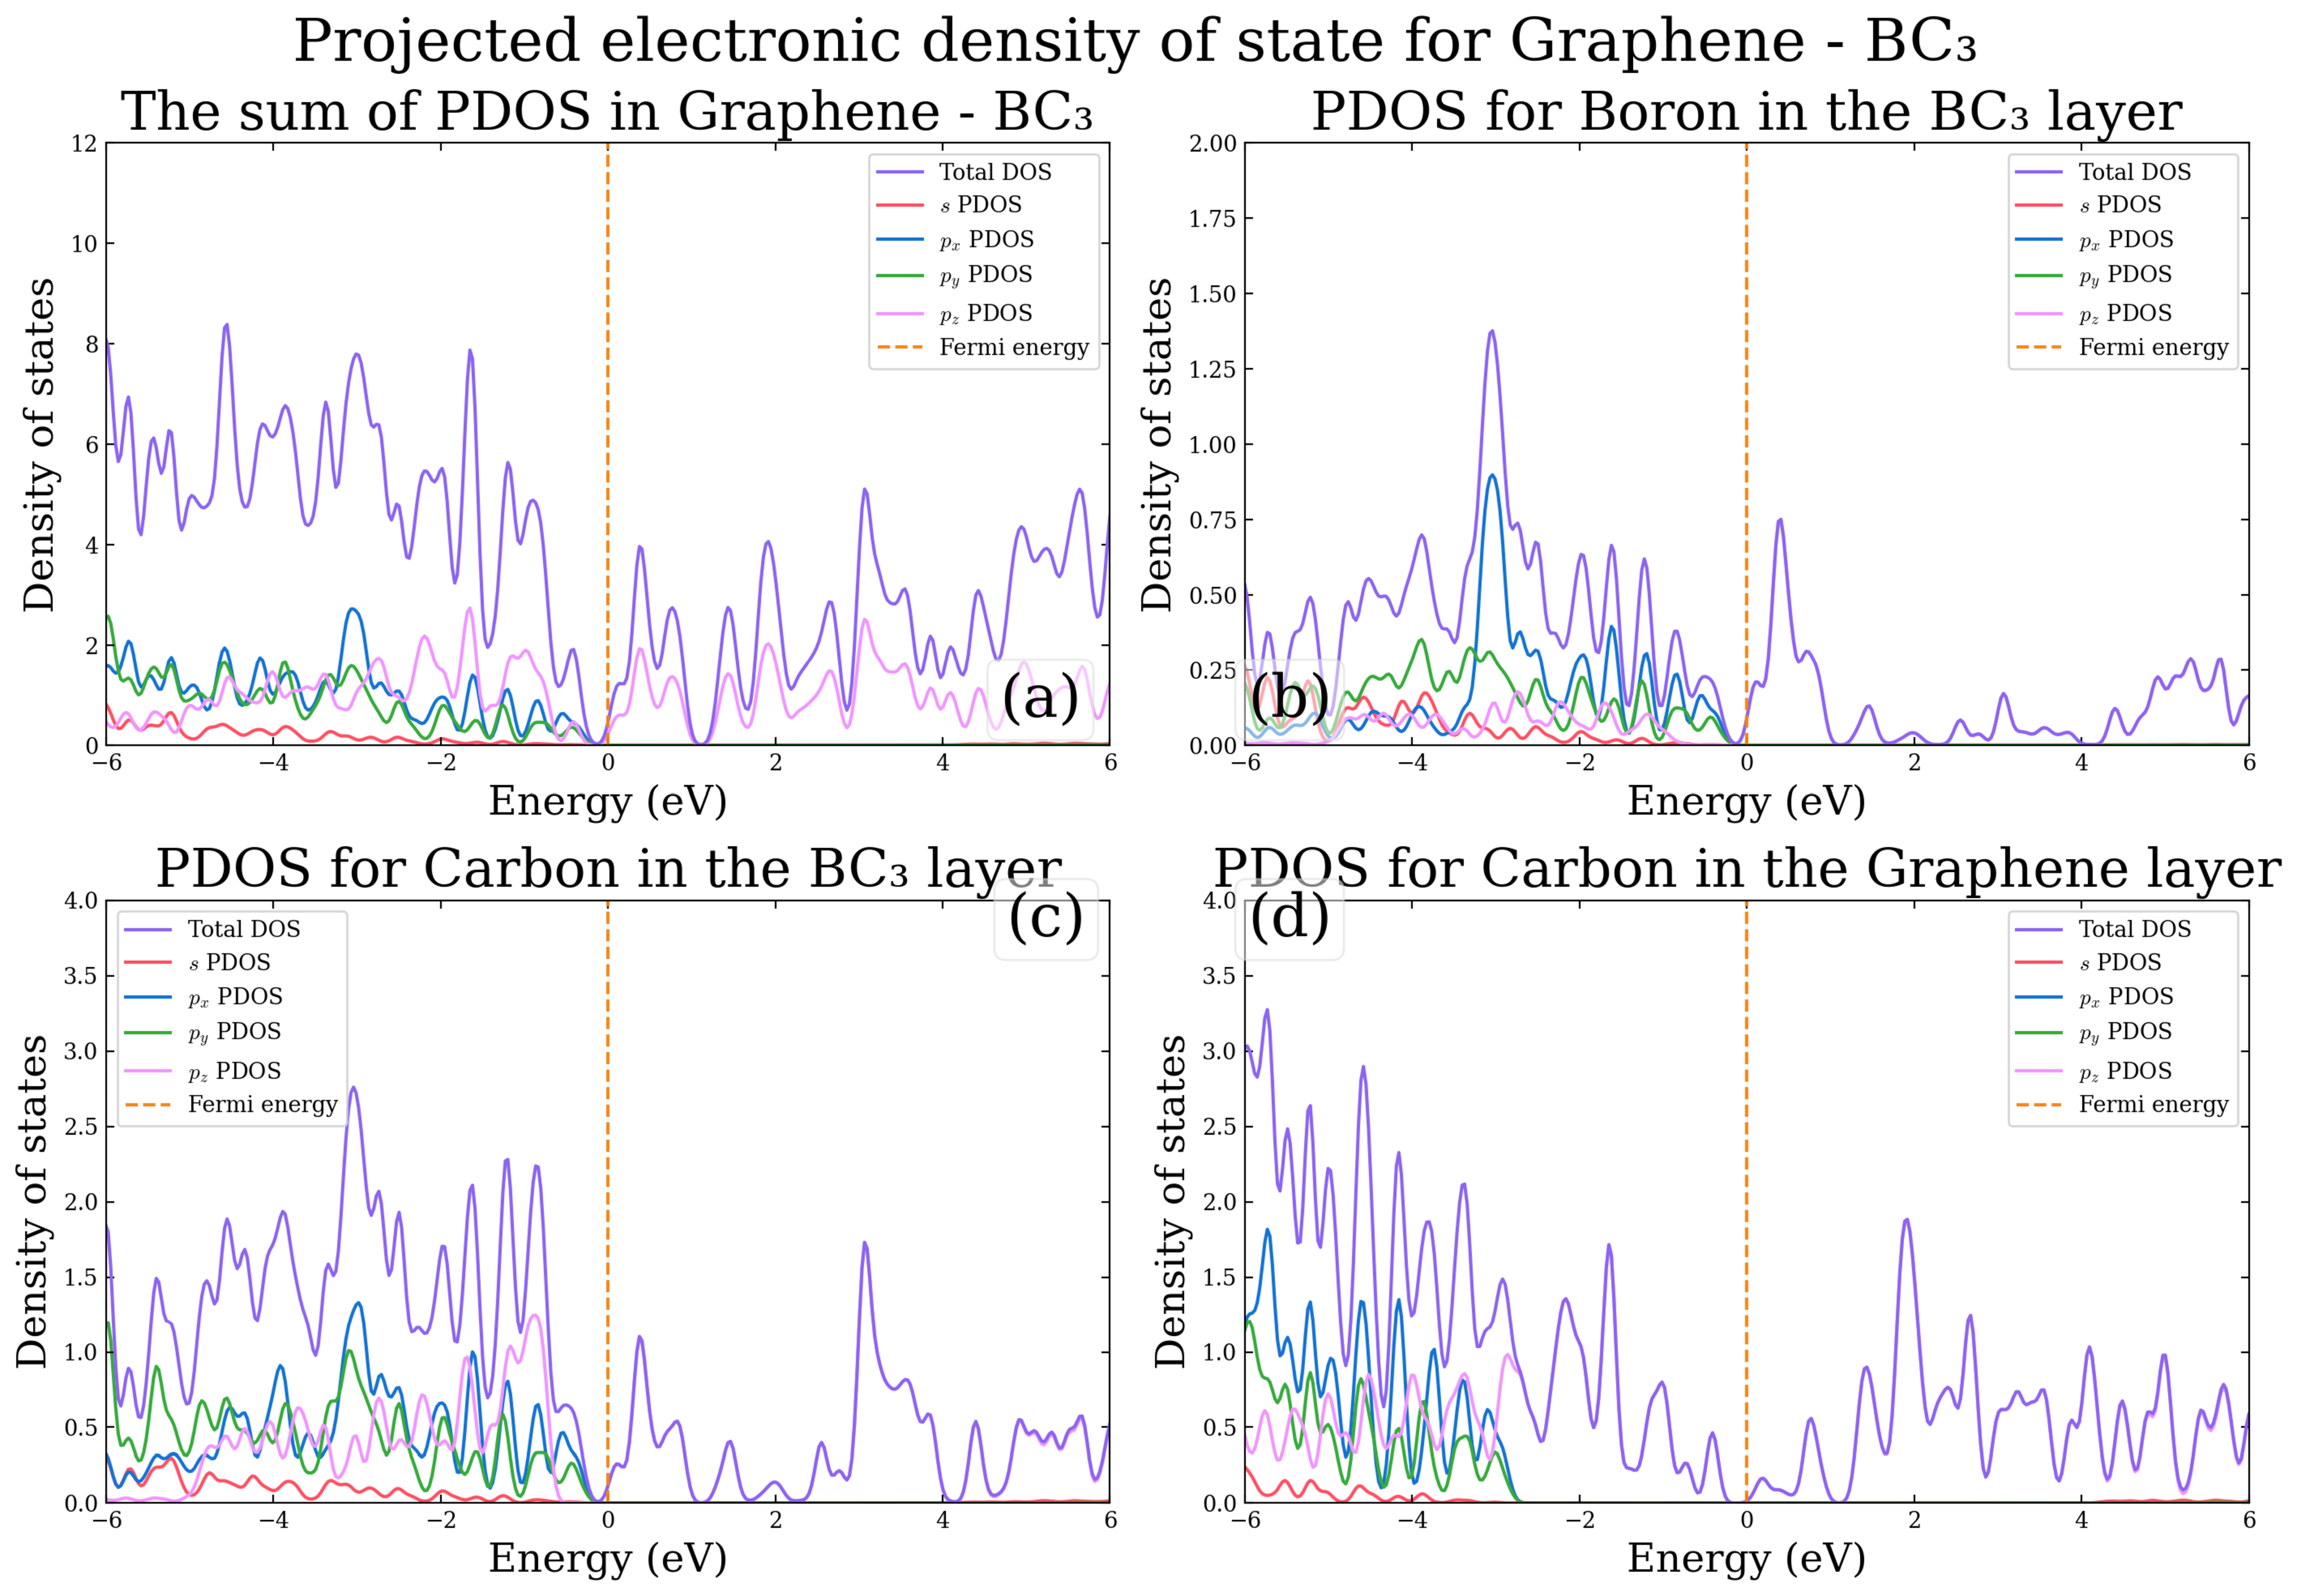
\includegraphics[width=0.30\linewidth]{poster_figures/G-BC3_PDOS.pdf}
    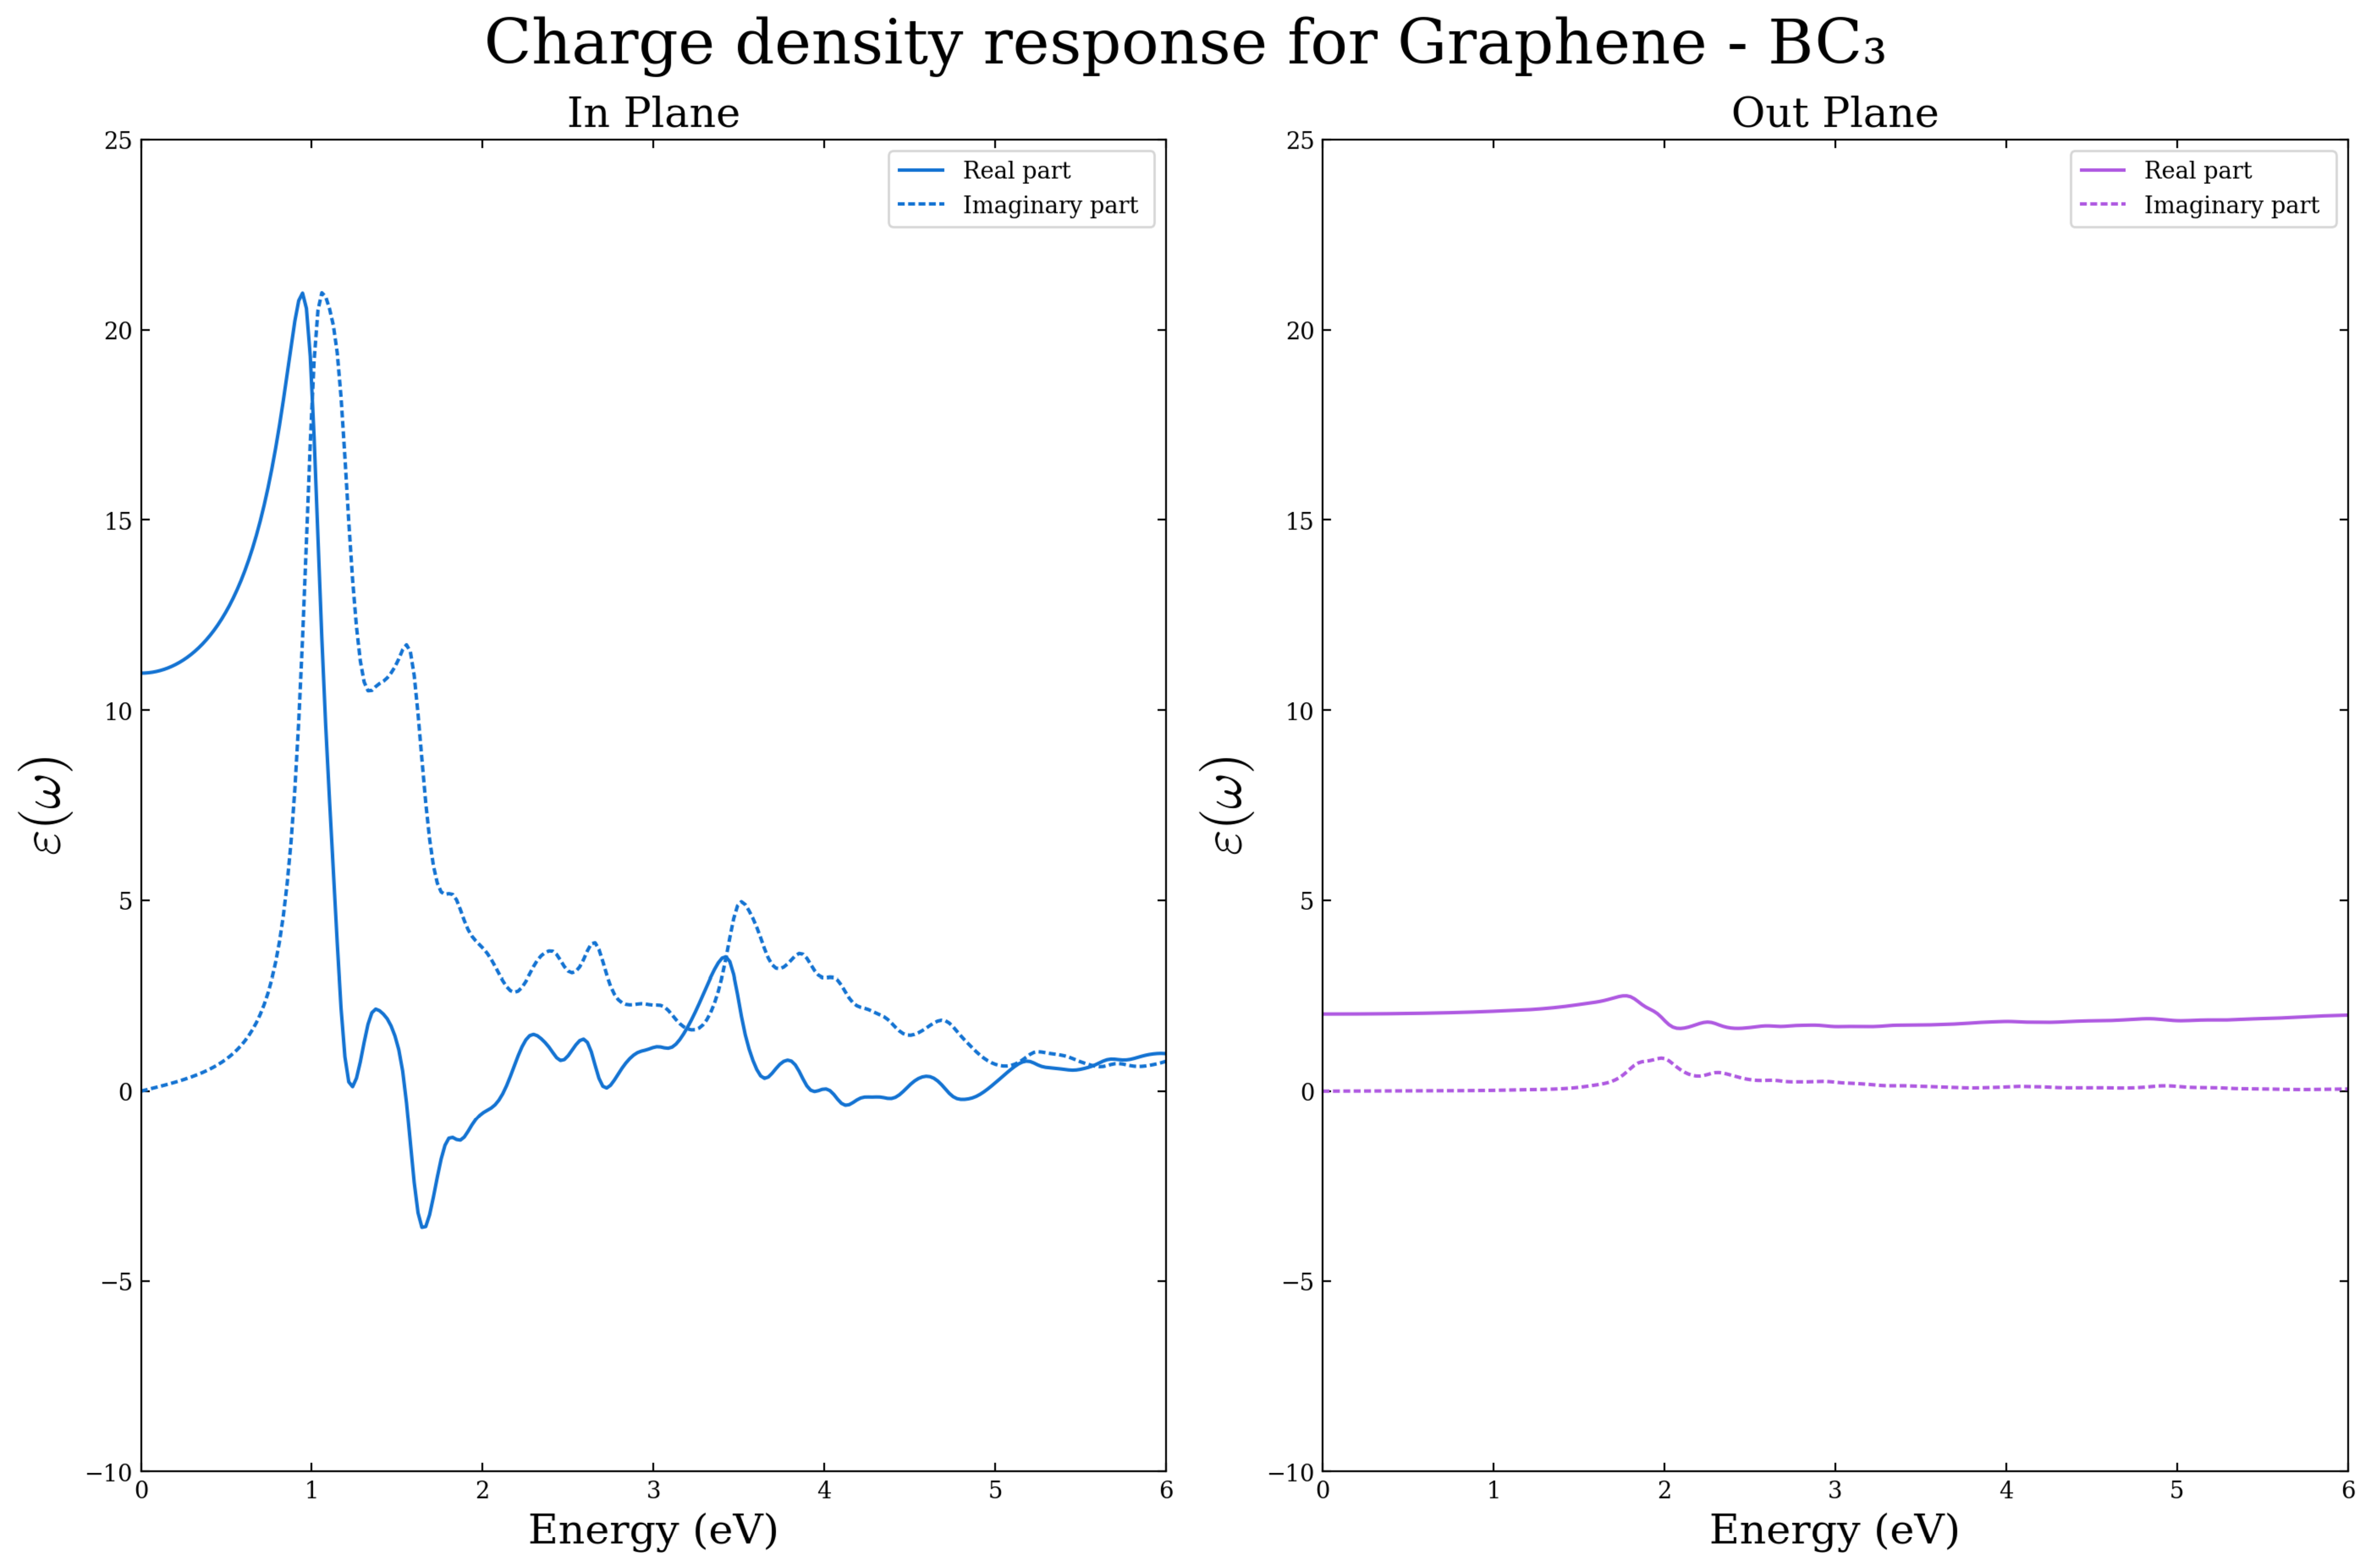
\includegraphics[width=0.30\linewidth]{poster_figures/G-BC3_opt.pdf}
\end{center}\end{minipage}

\vspace{0pt}\begin{minipage}{1\linewidth}\begin{center}\footnotesize
    \begin{tcolorbox}[colback=table_color_2, colframe=table_color_2, rounded corners, boxsep=2pt, left=0pt, right=0pt, top=0pt, bottom=0pt]
        \par $\bullet$ Interaction between Graphene and BC\textsubscript{3} layers results in possible metallic behaviour.
        \par $\bullet$ Low energy response dominated by characteristic BC3 peaks around 1 eV and 1.5 eV, graphene character is more prominent higher energies.
    \end{tcolorbox}
\end{center}\end{minipage}

\vspace{5pt}\begin{minipage}[t]{0.4\linewidth}
    \begin{center}
        \small\textcolor{dark_blue}{\textbf{Absorption Coefficient}}
        \vspace{-5pt}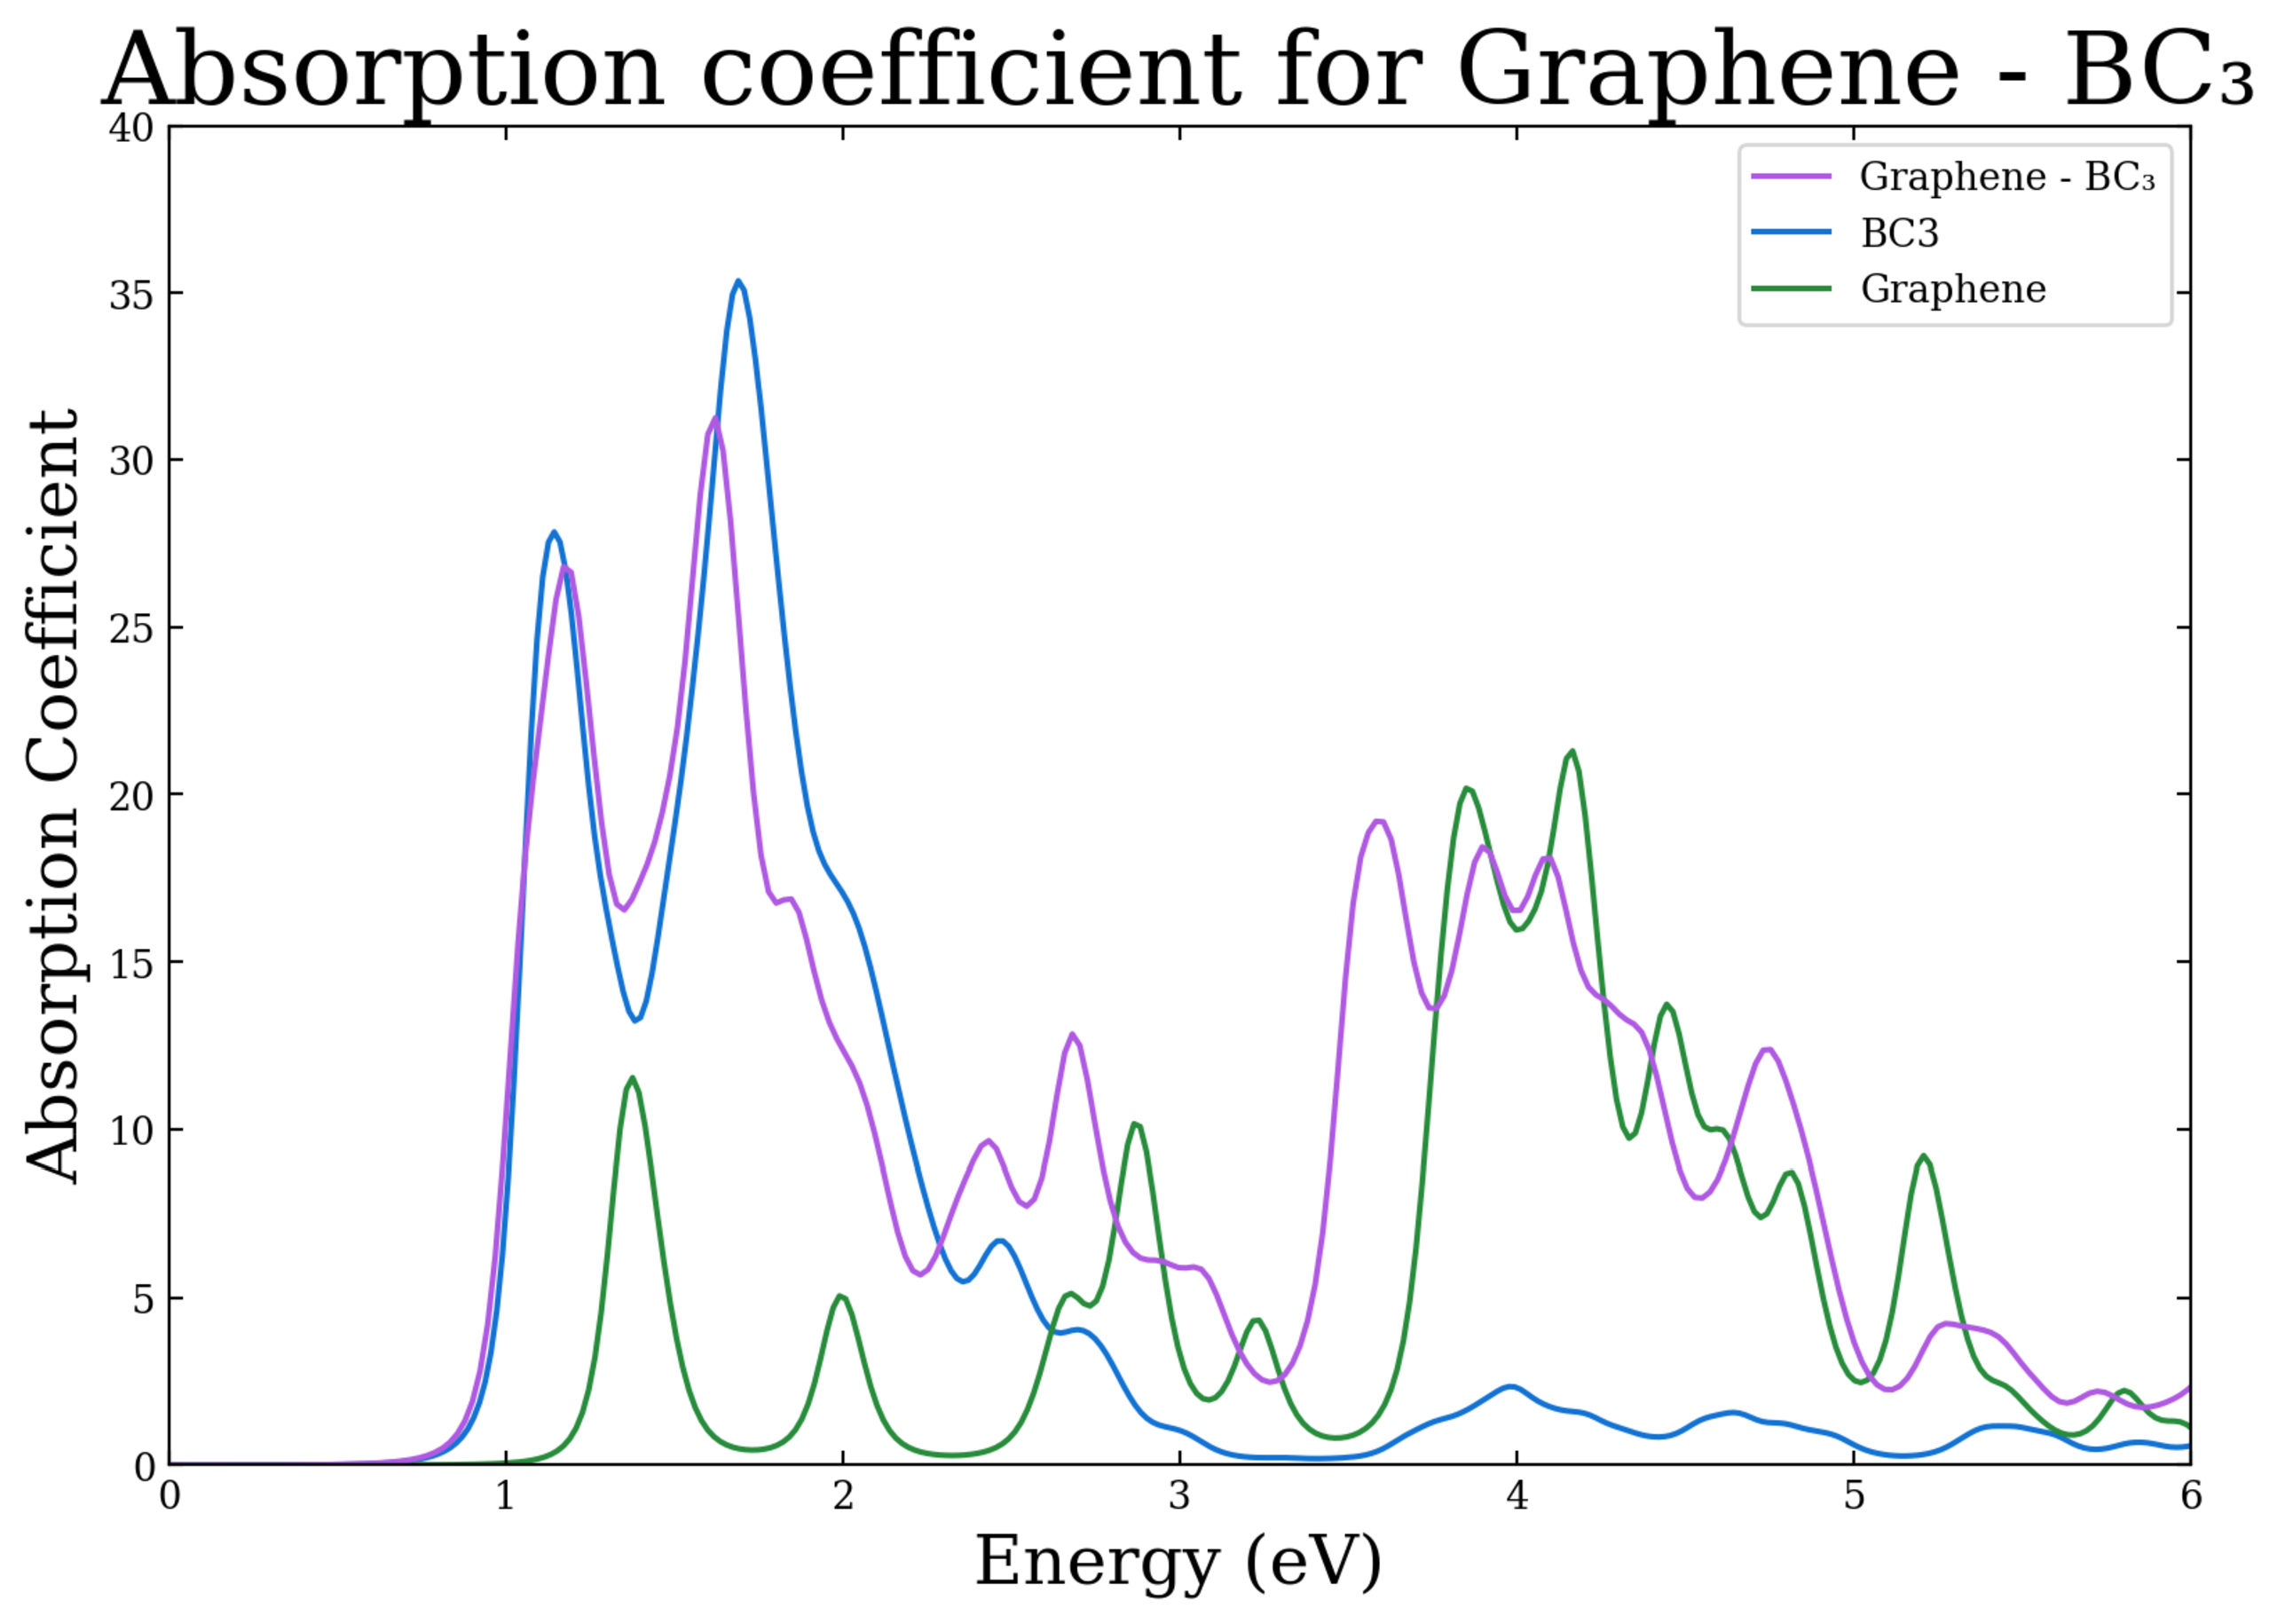
\includegraphics[width=0.8\linewidth]{poster_figures/AC.pdf}
    \end{center}
    \footnotesize{
        \vspace{-10pt}\begin{tcolorbox}[colback=table_color_2, colframe=table_color_2, rounded corners, boxsep=2pt, left=0pt, right=0pt, top=0pt, bottom=0pt]
            Characteristic adsorption peaks are found for G-BC3 around 1200nm, 700nm, and 450nm with a broader set of peaks in the UV between 350nm to 250nm.
            Peaks for G-BC3 are generally shifted to lower energies compared to Graphene.
        \end{tcolorbox}}
\end{minipage}
\begin{minipage}[t]{0.56\linewidth}
    \begin{center}
        \small\textcolor{dark_blue}{\textbf{Future Work}}
    \end{center}
    \footnotesize{
        \begin{tcolorbox}[colback=table_color_2, colframe=table_color_2, rounded corners, boxsep=2pt, left=0pt, right=0pt, top=0pt, bottom=0pt]
            \par $\bullet$ Future work comparative studies with HSE06 functional;
            \par $\bullet$ Further investigation will look at G-B\textsubscript{4}C\textsubscript{3}, G-B bilayers.
        \end{tcolorbox}}
    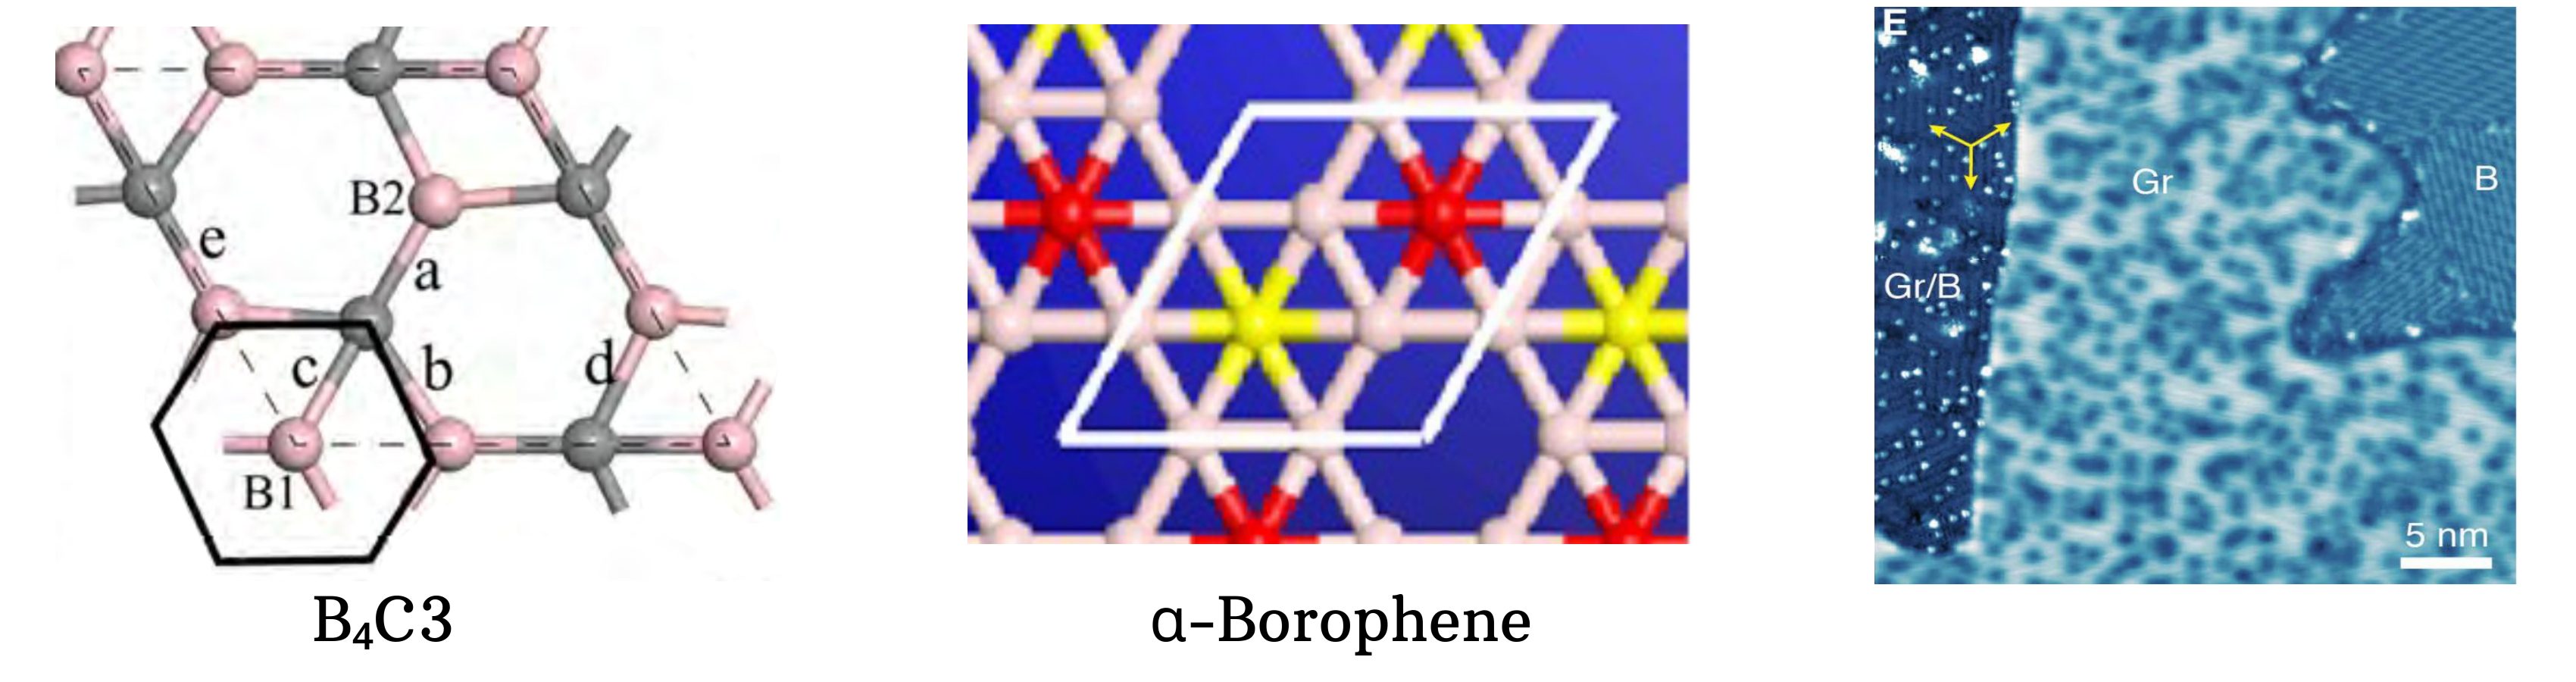
\includegraphics[width=1\linewidth]{poster_figures/Future.png}
    \footnotesize{
        \vspace{-10pt}\begin{tcolorbox}[colback=table_color_2, colframe=table_color_2, rounded corners, boxsep=2pt, left=0pt, right=0pt, top=0pt, bottom=0pt]
            Recently, Borophene and Graphene bilayer integration has been demonstrated experimentally;
            STM topography image of lateral and vertical heterostructures between borophene and graphene.
            Liu and Hersam, Sci. Adv. 2019; 5
        \end{tcolorbox}}
\end{minipage}

}

\headerbox{}{name=box_5, below=box_4, boxheaderheight=10pt, column=2, span=3}{
% \begin{minipage}[t]{0.4\linewidth}
%     \begin{center}
%         \small\textcolor{dark_blue}{\textbf{Conclusion}}
%     \end{center}
%     \vspace{-10}\footnotesize{
%         \par $\bullet$ Hollow site coordination is the favored configuration of the graphene-BC3 heterostructure.
%         \par $\bullet$ G-BC3 shows potentially metallic behavior, more work is needed to confirm these results, further optimization and more accurate functionals.
%         \par $\bullet$ Characteristic peaks adsorption peaks for G-BC3 have been identified. 
%     }
% \end{minipage}
\begin{minipage}[t]{0.4\linewidth}
    \begin{center}
        \small\textcolor{dark_blue}{\textbf{Conclusion}}
    \end{center}
    \vspace{-15}\footnotesize{
        \begin{tcolorbox}[colback=table_color_2, colframe=table_color_2, rounded corners, boxsep=2pt, left=0pt, right=0pt, top=0pt, bottom=0pt]
        \par $\bullet$ Hollow site coordination is the favored configuration of the graphene-BC3 heterostructure.
        \par $\bullet$ G-BC3 shows potentially metallic behavior, more work is needed to confirm these results, further optimization and more accurate functionals.
        \par $\bullet$ Characteristic peaks adsorption peaks for G-BC3 have been identified. 
        \end{tcolorbox}}
\end{minipage}
\begin{minipage}[t]{0.56\linewidth}
    \begin{center}
        \small\textcolor{dark_blue}{\textbf{Acknowledgements}}
    \end{center}
    \vspace{-15}\footnotesize{
        \begin{tcolorbox}[colback=table_color_2, colframe=table_color_2, rounded corners, boxsep=2pt, left=0pt, right=0pt, top=0pt, bottom=0pt]
            We gratefully acknowledge support from
            \par $\bullet$ The Australian Research Council;
            \par $\bullet$ The Australian Government's National Collaborative Research Infrastructure Strategy (NCRIS),
            with access to computational resources provided by the National Computational Infrastructure (NCI) through the National Computational Merit Allocation Scheme
        \end{tcolorbox}}
    \end{minipage}

\vspace{-10pt}\begin{center}\begin{minipage}[t]{0.6\linewidth}\footnotesize{
\begin{tcolorbox}[colback=color_me, colframe=color_me, rounded corners, boxsep=2pt, left=0pt, right=0pt, top=0pt, bottom=0pt]
    \begin{center}
        For further information
        \par Please contact Lu Niu: luke.niu@sydney.edu.au
    \end{center}
\end{tcolorbox}}
\end{minipage}\end{center}
}

\end{poster}

\end{document}
